% !TeX encoding = UTF-8
% ================================================================
% JEDEN PLIK ŹRÓDŁOWY DLA CODEXA — UZUPEŁNIENIA ROZDZIAŁÓW 4, 11 i 28
% ================================================================
% INSTRUKCJA DLA CODEXA:
% Plik zawiera TRZY ODRĘBNE fragmenty, oznaczone poniżej znacznikami
% "POCZĄTEK / KONIEC". Wstawiaj do skryptu WYŁĄCZNIE treść pomiędzy
% znacznikami, w odpowiednich rozdziałach; nie dodawaj całości
% jako jednego \input w jednym miejscu ani nie twórz trzech plików.
% Zastąp stare dopiski o tych tematach, zamiast powielać sekcje.
%
% Rozdział 4: po istniejącej uwadze o w_2, przed "Dalszą lekturą";
% istniejąca definicja struktury spinowej zostaje, ale skoryguj jej
% nazwę "wiązka spinorowa" i zapis iloczynu stowarzyszonego:
% S=P_{\mathrm{Spin}}\times_{\varrho}\Delta_n, gdzie \varrho to
% reprezentacja spinowa, a nie samo odwzorowanie nakrywające.
% Rozdział 11: bezpośrednio przed \section{Długość, energia i odległość}.
% Rozdział 28 (Teoria Hodge'a i metoda Bochnera): po wprowadzeniu
% laplasjanu Hodge'a i tożsamości Bochnera--Weitzenböcka, w pobliżu
% twierdzeń Cherna--Gaussa--Bonneta i Atiyaha--Singera.
%
% Zasady: wszystkie twierdzenia muszą mieć jawnie podane założenia;
% konsekwentnie używaj "ramka", "wiązka spinorowa", "pole spinorowe".
% Całki z miar: \dd\lambda_n(x) i \dd\mu_g(x), bez notacji fizycznej.
% Nie dołączaj \documentclass ani preambuły; istniejący dokument
% korzysta z amsmath, amssymb, amsthm, mathtools i tikz.
% ================================================================


%=====================================================================
% >>>>>>>>>>>>> CODEX: POCZĄTEK ROZDZIAŁU 4 — WIĄZKA SPINOROWA I POLE SPINOROWE
%=====================================================================

% UZUPEŁNIENIE ROZDZIAŁU 4: WIĄZKA SPINOROWA I POLE SPINOROWE
% Miejsce: po istniejącej uwadze o klasie w_2, przed "Dalszą lekturą".
% Istniejącą Definicję \ref{def:struktura-spinowa} zachować, ale poprawić
% nazwę "wiązka spinorowa" i niepoprawny indeks w iloczynie stowarzyszonym.
% Poniżej uściślamy konstrukcję i opisujemy warunki sklejania.
% Rozmaitość spinowa, warunek w_2(TM)=0 i przykłady: rozdział 11.
% Zachowujemy nazwę "ramka", a nie "rama".

\section{Wiązka spinorowa i pole spinorowe}
\label{sec:pola-spinorowe-podstawy}

W poprzednich częściach rozdziału skonstruowaliśmy algebrę Clifforda,
grupę $\operatorname{Spin}(n)$, jej reprezentacje i strukturę spinową. Teraz przechodzimy od spinoru jako elementu pojedynczej
przestrzeni wektorowej do spinorów zmieniających się gładko na
rozmaitości. Istotne jest rozróżnienie \emph{włókna spinorowego},
\emph{wiązki spinorowej} i \emph{pola spinorowego}. Kwestia tego,
kiedy rozmaitość dopuszcza strukturę spinową, zostanie rozwinięta
w Rozdziale~\ref{ch:metryka-riemannowska},
w Sekcji~\ref{sec:rozmaitosci-spinowe}.

Niech $(M^n,g)$ będzie zorientowaną rozmaitością riemannowską,
na której wybrano strukturę spinową
$P_{\mathrm{Spin}}\to M$ z Definicji~\ref{def:struktura-spinowa}.
Niech $\Delta_n$ oznacza nieredukowalny zespolony moduł algebry
$\operatorname{Cl}^{\mathbb C}_n$, a
$\varrho:\operatorname{Spin}(n)\to\operatorname{GL}(\Delta_n)$
reprezentację spinową. Elementy włókien $P_{\mathrm{Spin}}$
będziemy nazywać \emph{ramkami spinowymi}; ich obrazy
w wiązce ramek ortonormalnych to zwykłe ramki geometryczne.

\begin{definicja}[Wiązka spinorowa i pole spinorowe]
\label{def:pole-spinorowe-globalne}
Niech $n\geq2$, niech $(M^n,g)$ będzie zorientowaną rozmaitością
riemannowską z wybraną strukturą spinową $P_{\mathrm{Spin}}\to M$.
Niech $\Delta_n$ będzie ustalonym nieredukowalnym zespolonym
modułem $\operatorname{Cl}^{\mathbb C}_n$, a
$\varrho:\operatorname{Spin}(n)\to\operatorname{GL}(\Delta_n)$
odpowiadającą mu reprezentacją spinową.
\emph{Zespolona wiązka spinorowa} stowarzyszona
z wybraną strukturą spinową jest wiązką wektorową
\begin{equation}\label{eq:pola-spinorowe-wiazka}
 S(M):=P_{\mathrm{Spin}}\times_{\varrho}\Delta_n
 =\bigl(P_{\mathrm{Spin}}\times\Delta_n\bigr)/{\sim},
 \qquad (ph,z)\sim(p,\varrho(h)z).
\end{equation}
\emph{Spinor w punkcie} $x\in M$ jest elementem włókna
$S_x(M)$. \emph{Polem spinorowym} jest gładki przekrój
$\psi\in\Gamma^\infty(S(M))$, czyli gładkie odwzorowanie
$\psi:M\to S(M)$, dla którego
$\pi_S\circ\psi=\operatorname{id}_M$.
\end{definicja}

W szczególności globalnego pola nie można utożsamiać z jedną
kolumną funkcji o wartościach w $\mathbb C^N$, o ile nie
wybrano globalnej trywializacji wiązki. W lokalnej ramce
spinowej pole jest reprezentowane przez kolumnę, która
przy zmianie ramki podlega określonemu prawu transformacji.

\begin{stwierdzenie}[Lokalny opis pola i warunek sklejania]
\label{prop:pola-spinorowe-sklejanie}
Niech $n\geq2$, niech $(M^n,g)$ będzie zorientowaną rozmaitością
riemannowską z wybraną strukturą spinową
$P_{\mathrm{Spin}}\to M$, a $S(M)$ stowarzyszoną
wiązką spinorową z Definicji~\ref{def:pole-spinorowe-globalne}.
Niech $(U_i)$ będzie pokryciem $M$ oraz
$s_i:U_i\to P_{\mathrm{Spin}}$ jego gładkimi lokalnymi
przekrojami. Na $U_i\cap U_j$ określmy
$h_{ij}:U_i\cap U_j\to\operatorname{Spin}(n)$ przez
$s_j=s_i h_{ij}$ i połóżmy $R_{ij}=\varrho(h_{ij})$.
Pole spinorowe $\psi$ ma na $U_i$ jednoznaczny zapis
$\psi(x)=[s_i(x),\psi_i(x)]$, gdzie $\psi_i:U_i\to\Delta_n$
są gładkie i spełniają
\begin{equation}\label{eq:pola-spinorowe-przejscie}
 \psi_i=R_{ij}\psi_j\qquad\text{na }U_i\cap U_j.
\end{equation}
Odwrotnie, każda rodzina gładkich funkcji $\psi_i$
spełniających ten warunek wyznacza dokładnie jedno globalne
pole spinorowe.
\end{stwierdzenie}
\begin{proof}
Z definicji ilorazu otrzymujemy
$[s_j,\psi_j]=[s_i h_{ij},\psi_j]
=[s_i,\varrho(h_{ij})\psi_j]$.
Wobec jednoznaczności współrzędnych w lokalnej
trywializacji równość ta jest równoważna
$\psi_i=R_{ij}\psi_j$. Odwrotnie, wzory
$\psi(x)=[s_i(x),\psi_i(x)]$ nie zależą wówczas od wyboru
$i$ na przecięciach obszarów, a lokalna gładkość daje
gładkość globalną.
\end{proof}

\begin{stwierdzenie}[Pola jako odwzorowania ekwiwariantne]
\label{prop:pola-spinorowe-ekwiwariantnosc}
Niech $n\geq2$, niech $(M^n,g)$ będzie zorientowaną
rozmaitością riemannowską ze strukturą spinową
$P_{\mathrm{Spin}}\to M$, a $S(M)$ stowarzyszoną
wiązką spinorową określoną przez reprezentację
$\varrho:\operatorname{Spin}(n)\to\operatorname{GL}(\Delta_n)$.
Istnieje naturalna bijekcja między
$\Gamma^\infty(S(M))$ a zbiorem gładkich odwzorowań
$F:P_{\mathrm{Spin}}\to\Delta_n$ spełniających
\begin{equation}\label{eq:pola-spinorowe-ekwiwariantnosc}
 F(ph)=\varrho(h)^{-1}F(p),\qquad
 h\in\operatorname{Spin}(n),\quad p\in P_{\mathrm{Spin}}.
\end{equation}
\end{stwierdzenie}
\begin{proof}
Dla pola $\psi$ i ramki spinowej $p$ nad $x$ istnieje
jedyny $z\in\Delta_n$ taki, że $\psi(x)=[p,z]$;
kładziemy $F(p)=z$. Przejście do $ph$ wymusza
$F(ph)=\varrho(h)^{-1}F(p)$. Odwrotnie, dla takiego $F$
przypisanie $x\mapsto[p,F(p)]$ nie zależy od wyboru
ramki nad $x$ i wyznacza gładki przekrój.
\end{proof}

\begin{uwaga}[Ramki ortonormalne a ramki spinowe]
\label{rem:pola-spinorowe-ramki}
Niech na przecięciu $e_j=e_i A_{ij}$ oznacza zmianę
lokalnej ramki ortonormalnej, gdzie $A_{ij}$ jest
odwzorowaniem o wartościach w $\mathrm{SO}(n)$,
a $h_{ij}$ jego podniesieniem do $\operatorname{Spin}(n)$.
Współrzędne wektora stycznego transformują się jako
$v_j=A_{ij}^{-1}v_i$, natomiast współrzędne spinora
jako $\psi_j=\varrho(h_{ij})^{-1}\psi_i$.
Są to działania różnych reprezentacji. W szczególności
wektor nie staje się spinorem tylko dlatego, że zapisano go
w postaci kolumny współrzędnych.
\end{uwaga}

\begin{center}
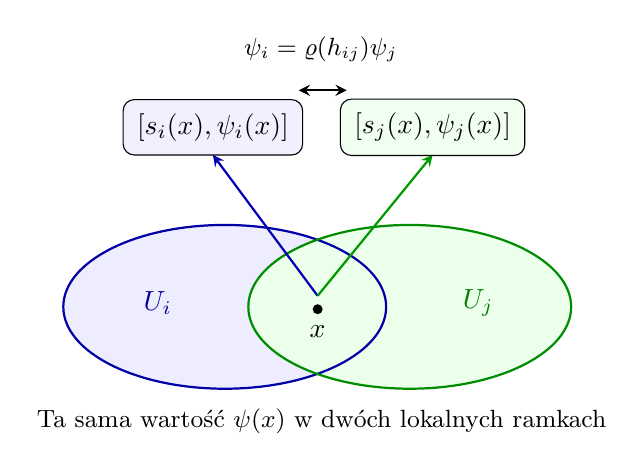
\begin{tikzpicture}[>=stealth,scale=1]
 \fill[blue!7] (-4.7,-1.1) ellipse (2.05 and 1.04);
 \fill[green!8] (-2.35,-1.1) ellipse (2.05 and 1.04);
 \draw[blue!65!black,thick] (-4.7,-1.1) ellipse (2.05 and 1.04);
 \draw[green!55!black,thick] (-2.35,-1.1) ellipse (2.05 and 1.04);
 \fill[black] (-3.52,-1.13) circle (1.8pt);
 \node[below] at (-3.52,-1.22) {$x$};
 \node[blue!60!black] at (-5.55,-1.05) {$U_i$};
 \node[green!50!black] at (-1.48,-1.05) {$U_j$};
 \draw[->,thick,blue!70!black] (-3.52,-.96)--(-4.85,.83);
 \draw[->,thick,green!60!black] (-3.52,-.96)--(-2.06,.83);
 \node[draw,rounded corners,fill=blue!6,align=center,inner sep=5pt]
  at (-4.85,1.18) {$[s_i(x),\psi_i(x)]$};
 \node[draw,rounded corners,fill=green!6,align=center,inner sep=5pt]
  at (-2.06,1.18) {$[s_j(x),\psi_j(x)]$};
 \draw[<->,thick] (-3.76,1.65)--(-3.15,1.65);
 \node[font=\small] at (-3.48,2.17)
  {$\psi_i=\varrho(h_{ij})\psi_j$};
 \node[font=\small] at (-3.47,-2.55)
  {Ta sama wartość $\psi(x)$ w dwóch lokalnych ramkach};
\end{tikzpicture}

{\small\itshape Dwie lokalne reprezentacje jednego pola spinorowego.
Warunek sklejania zapewnia zgodność na przecięciu map.}
\end{center}

\begin{uwaga}[Pełny obrót ramki]
Dwa elementy $h$ i $-h$ mają ten sam obraz
w $\mathrm{SO}(n)$, lecz na nieredukowalnym module
spinowym działają przeciwnie. Dlatego podniesienie
pełnego obrotu o $2\pi$ może zmienić znak spinora,
chociaż sam obrót jest tożsamością na wektorach.
Nie oznacza to, że pojedynczy spinor jest wektorem
w innej bazie; stanowi on element innej reprezentacji.
\end{uwaga}

\subsection{Mnożenie Clifforda i półspinory}

\begin{stwierdzenie}[Globalne działanie Clifforda]
\label{prop:pola-spinorowe-clifford}
Niech $n\geq2$, niech $(M^n,g)$ będzie zorientowaną
rozmaitością riemannowską z wybraną strukturą spinową,
a $S(M)$ stowarzyszoną zespoloną wiązką spinorową.
Na $S(M)$ istnieje naturalne, gładkie, włóknowo dwuliniowe
działanie $c:TM\otimes S(M)\to S(M)$ takie, że
\begin{equation}\label{eq:pola-spinorowe-clifford}
 c(v)c(w)+c(w)c(v)=-2g(v,w)I_{S_x},
 \qquad v,w\in T_xM.
\end{equation}
Jeśli $n$ jest parzyste, istnieje rozkład
$S(M)=S^+(M)\oplus S^-(M)$ na wiązki półspinorowe.
\end{stwierdzenie}
\begin{proof}
W lokalnej ramce ortonormalnej działanie na włóknie
identyfikujemy z reprezentacją Clifforda na $\Delta_n$.
Dla $h\in\operatorname{Spin}(n)$ zachodzi
$\varrho(h)c(v)\varrho(h)^{-1}=c(\rho(h)v)$,
gdzie $\rho:\operatorname{Spin}(n)\to\mathrm{SO}(n)$
jest standardowym nakryciem, a $v\in\mathbb R^n$.
Jest to dokładnie zgodność wymagana do sklejenia
działań lokalnych. W wymiarze parzystym operator
chiralności $\Gamma$ z~\ref{prop:spin-chiral} komutuje
z $\varrho(h)$; jego przestrzenie własne są więc
podprzestrzeniami niezmienniczymi i wyznaczają
podwiązki $S^\pm(M)$.
\end{proof}

\begin{definicja}[Pełne pole spinorowe i pole półspinorowe]
\label{def:pola-spinorowe-dirac-weyl}
Niech $n\geq2$ i niech $S(M)$ będzie zespoloną wiązką
spinorową z Definicji~\ref{def:pole-spinorowe-globalne}.
Polem spinorowym pełnym nazywamy gładki przekrój $S(M)$.
Gdy $n$ jest parzyste, \emph{polem półspinorowym}
(chiralnym) nazywamy przekrój jednej z wiązek
$S^+(M)$ lub $S^-(M)$. Rozkład
$\psi=\psi_++\psi_-$ jest określony geometrycznie,
niezależnie od wyboru lokalnej ramki.
W czasoprzestrzeni lorentzowskiej odpowiada to
rozróżnieniu pól Diraca i Weyla; omówimy je
w Sekcji~\ref{sec:rozmaitosci-spinowe}.
\end{definicja}

\begin{przyklad}[Pola na płaskim torusie]
\label{prz:pola-spinorowe-torus}
Rozważmy $T^2=\mathbb R^2/(2\pi\mathbb Z)^2$.
Po wyborze struktury spinowej periodycznej w obu
kierunkach pole spinorowe można przedstawić przez
$\psi:\mathbb R^2\to\mathbb C^2$ spełniającą
$\psi(x+2\pi,y)=\psi(x,y)$ oraz
$\psi(x,y+2\pi)=\psi(x,y)$. Jeśli struktura
jest antyperiodyczna wzdłuż pierwszego generatora,
pierwszy warunek zastępuje
$\psi(x+2\pi,y)=-\psi(x,y)$.
Nie jest to wielowartościowość pola na torusie,
lecz skutek innego sklejenia włókien wiązki spinorowej.
\end{przyklad}

\subsection{Koneksja spinorowa i zmiana ramki}

Dla lokalnych zapisów $\psi_i=R_{ij}\psi_j$ pochodna
zewnętrzna spełnia
$\dd\psi_i=(\dd R_{ij})\psi_j+R_{ij}\dd\psi_j$.
Dodatkowy składnik nie pozwala skleić zwykłych
pochodnych kolumn w globalny przekrój
$T^*M\otimes S(M)$. Potrzebujemy koneksji.

\begin{stwierdzenie}[Prawo transformacji koneksji]
\label{prop:pola-spinorowe-transformacja-koneksji}
Niech $n\geq2$, niech $(M^n,g)$ będzie zorientowaną
rozmaitością riemannowską ze strukturą spinową,
niech $S(M)$ będzie stowarzyszoną wiązką spinorową
i niech $\nabla^S$ będzie koneksją w $S(M)$.
Niech $(U_i)$ będzie pokryciem trywializującym,
a $R_{ij}:U_i\cap U_j\to\operatorname{GL}(\Delta_n)$
macierzami przejścia współrzędnych spinorów, tzn.
$\psi_i=R_{ij}\psi_j$ na $U_i\cap U_j$.
Jeśli na $U_i$ ma lokalną postać
$(\nabla^S\psi)_i=\dd\psi_i+A_i^S\psi_i$,
gdzie $A_i^S\in\Omega^1(U_i;\operatorname{End}\Delta_n)$,
to na przecięciu $U_i\cap U_j$ zachodzi
\begin{equation}\label{eq:pola-spinorowe-transformacja-koneksji}
 A_j^S=R_{ij}^{-1}A_i^SR_{ij}+R_{ij}^{-1}\dd R_{ij}.
\end{equation}
Odwrotnie, rodzina lokalnych form macierzowych
spełniających tę relację określa globalną koneksję.
\end{stwierdzenie}
\begin{proof}
Z równości $\psi_i=R_{ij}\psi_j$ oraz
$(\nabla^S\psi)_i=R_{ij}(\nabla^S\psi)_j$
wynika
\[
 (\dd R_{ij})\psi_j+R_{ij}\dd\psi_j
   +A_i^SR_{ij}\psi_j
 =R_{ij}\dd\psi_j+R_{ij}A_j^S\psi_j.
\]
Skrócenie składników zawierających $\dd\psi_j$
i pomnożenie z lewej przez $R_{ij}^{-1}$ daje
żądany wzór. W odwrotną stronę ten sam rachunek
wykazuje zgodność lokalnych pochodnych kowariantnych,
a więc pozwala je skleić.
\end{proof}

\begin{uwaga}[Koneksja zgodna ze strukturą spinową]
Koneksję Leviego--Civity można podnieść z wiązki
ramek ortonormalnych na wiązkę spinową. Jej działanie
przez reprezentację $\varrho$ określa wyróżnioną
koneksję spinorową. Wzór lokalny i operator
$D=\sum_jc(e_j)\nabla^S_{e_j}$ wyprowadzimy
w Sekcji~\ref{subsec:dirac-koneksja}.
\end{uwaga}

% <<<<<<<<<<<<< CODEX: KONIEC ROZDZIAŁU 4


%=====================================================================
% >>>>>>>>>>>>> CODEX: POCZĄTEK ROZDZIAŁU 11 — ROZMAITOŚCI SPINOWE
%=====================================================================

% UZUPELNIENIE ROZDZIALU 11 -- WERSJA PO KONTROLI PRECYZJI
% Umiescic bezposrednio przed \section{Długość, energia i odległość}.
% Korzysta z definicji grupy Spin(n), ramki ortonormalnej i wiazki glownej
% z rozdzialu 4, ale wszystkie oznaczenia w twierdzeniach ustala ponownie.
% Nie wymaga klas Cherna (pojawiaja sie w pozniejszym rozdziale).

\section{Rozmaitości spinowe}
\label{sec:rozmaitosci-spinowe}

W Rozdziale~\ref{ch:grass-spin} wprowadziliśmy algebrę Clifforda,
grupę $\operatorname{Spin}(n)$ oraz pojęcie struktury spinowej
na zorientowanej wiązce euklidesowej. Tutaj zastosujemy tę konstrukcję
do wiązki stycznej rozmaitości. Zaczniemy od definicji, następnie
skonstruujemy przeszkodę topologiczną do istnienia struktury spinowej
i zbadamy jednoznaczność jej wyboru. Odwołania do wcześniejszego
rozdziału wskazują pochodzenie konstrukcji, lecz założenia i oznaczenia
w poniższych twierdzeniach będziemy każdorazowo ustalać jawnie.

\begin{definicja}[Rozmaitość spinowa]
\label{def:rozmaitosc-spinowa}
Niech $n\geq2$, niech $M$ będzie gładką rozmaitością wymiaru $n$
z ustaloną orientacją, a $g$ metryką riemannowską na $M$.
Oznaczmy przez $F^+_g(M)\to M$ wiązkę główną dodatnio
zorientowanych ramek $g$-ortonormalnych, której grupą
strukturalną jest $\mathrm{SO}(n)$. Niech
$\rho_n:\operatorname{Spin}(n)\to\mathrm{SO}(n)$
będzie standardowym dwukrotnym nakryciem grup Liego.

\emph{Strukturą spinową} na $(M,g)$ nazywamy parę
$\mathfrak s=(P_{\mathrm{Spin}},\lambda)$, gdzie
$P_{\mathrm{Spin}}\to M$ jest wiązką główną o grupie
$\operatorname{Spin}(n)$, a
$\lambda:P_{\mathrm{Spin}}\to F^+_g(M)$ jest gładkim
odwzorowaniem wiązek nad $\operatorname{id}_M$, spełniającym
$\lambda(ph)=\lambda(p)\rho_n(h)$ dla każdego
$p\in P_{\mathrm{Spin}}$ i każdego $h\in\operatorname{Spin}(n)$.
Na każdym włóknie $\lambda$ jest wówczas dwukrotnym nakryciem.

\emph{Riemannowską rozmaitością spinową} nazywamy czwórkę
$(M,g,\mathfrak o,\mathfrak s)$, gdzie $\mathfrak o$
stanowi wybraną orientację $M$, a $\mathfrak s$ strukturę
spinową względem $g$ i $\mathfrak o$. Powiemy, że
zorientowana rozmaitość $M$ \emph{dopuszcza strukturę spinową},
jeżeli istnieje przynajmniej jedna taka $\mathfrak s$.
\end{definicja}

Dwie struktury spinowe $\mathfrak s_1=(P_1,\lambda_1)$
i $\mathfrak s_2=(P_2,\lambda_2)$ na tym samym
$(M,g,\mathfrak o)$ nazywamy \emph{izomorficznymi},
jeśli istnieje izomorfizm wiązek głównych
$\Phi:P_1\to P_2$ nad $\operatorname{id}_M$ taki,
że $\lambda_2\circ\Phi=\lambda_1$. Nie wystarcza więc
izomorfizm samych wiązek $P_1$ i $P_2$ bez uwzględnienia
odwzorowań $\lambda_1,\lambda_2$.

\subsection{Druga klasa Stiefela--Whitneya}

W celu określenia przeszkody do istnienia struktury spinowej
przypomnijmy konstrukcję z Rozdziału~\ref{ch:grass-spin}
i zapiszmy ją dla dowolnej zorientowanej wiązki euklidesowej.
Nie będziemy tu traktować symbolu $w_2$ jako niezdefiniowanego
skrótu.

\begin{definicja}[Druga klasa Stiefela--Whitneya]
\label{def:spin-w2}
Niech $M$ będzie gładką rozmaitością, a $E\to M$
zorientowaną rzeczywistą wiązką wektorową rzędu
$n\geq2$, wyposażoną w gładki iloczyn skalarny
we włóknach. Wybierzmy dobre pokrycie otwarte
$\mathcal U=(U_i)_{i\in I}$ rozmaitości $M$, tzn.
pokrycie, którego każde niepuste skończone przecięcie
jest ściągalne, oraz dodatnio zorientowane ortonormalne
ramki $e_i$ wiązki $E$ na $U_i$.

Na $U_i\cap U_j$ niech $g_{ij}:U_i\cap U_j\to\mathrm{SO}(n)$
będzie jedyną funkcją spełniającą $e_j=e_i g_{ij}$.
Wówczas $g_{ij}g_{jk}=g_{ik}$ na potrójnych przecięciach.
Dla każdego niepustego $U_i\cap U_j$ wybierzmy gładkie
podniesienie $h_{ij}:U_i\cap U_j\to\operatorname{Spin}(n)$
takie, że $\rho_n\circ h_{ij}=g_{ij}$,
$h_{ii}=1$ i $h_{ji}=h_{ij}^{-1}$. Istnieje ono, ponieważ
$U_i\cap U_j$ jest ściągalne.

Na niepustym potrójnym przecięciu kładziemy
\begin{equation}\label{eq:spin-w2-cocycle}
 \varepsilon_{ijk}=h_{ij}h_{jk}h_{ki}\in\{1,-1\}.
\end{equation}
Utożsamiamy $\{1,-1\}$ z addytywną grupą
$\mathbb Z/2$ przez $1\mapsto0$ i $-1\mapsto1$.
Układ $(\varepsilon_{ijk})$ wyznacza dwukocykl \v{C}ech
ze współczynnikami w $\mathbb Z/2$. Jego klasę
w $\check H^2(\mathcal U;\mathbb Z/2)$, utożsamioną
z $H^2(M;\mathbb Z/2)$ za pomocą dobrego pokrycia,
nazywamy \emph{drugą klasą Stiefela--Whitneya wiązki $E$}
i oznaczamy przez $w_2(E)$.
\end{definicja}

\begin{stwierdzenie}[Poprawność definicji $w_2(E)$]
\label{prop:spin-w2-dobrze-okreslona}
Niech $M$ będzie gładką rozmaitością, a $E\to M$
zorientowaną rzeczywistą wiązką wektorową rzędu $n\geq2$.
Klasa $w_2(E)\in H^2(M;\mathbb Z/2)$ z
Definicji~\ref{def:spin-w2} nie zależy od wyboru
metryki we włóknach, dobrego pokrycia, lokalnych ramek
ortonormalnych ani podniesień funkcji przejścia.
\end{stwierdzenie}
\begin{proof}
Niech $g_{ij}$ i $h_{ij}$ mają znaczenie ustalone
w Definicji~\ref{def:spin-w2}. Ponieważ
$\rho_n(h_{ij}h_{jk}h_{ki})=g_{ij}g_{jk}g_{ki}=I_n$,
każda funkcja $\varepsilon_{ijk}$ przyjmuje wartości
w centralnym jądrze $\ker\rho_n=\{\pm1\}$.
Z równości $h_{ij}h_{jk}=\varepsilon_{ijk}h_{ik}$
i łączności mnożenia otrzymujemy na poczwórnych
przecięciach
$\varepsilon_{ijk}\varepsilon_{ik\ell}
=\varepsilon_{jk\ell}\varepsilon_{ij\ell}$.
Jest to warunek dwukocyklu.

Inny wybór podniesień tych samych funkcji przejścia
ma postać $h'_{ij}=\delta_{ij}h_{ij}$, gdzie
$\delta_{ij}:U_i\cap U_j\to\{\pm1\}$ jest lokalnie stała,
$\delta_{ji}=\delta_{ij}^{-1}$. Wtedy
$\varepsilon'_{ijk}=\delta_{ij}\delta_{jk}\delta_{ki}
\varepsilon_{ijk}$, więc obydwa dwukocykle różnią się
o kobrzeg jedynokołańcucha $\delta=(\delta_{ij})$
w kompleksie kołańcuchów \v{C}ech.

Jeśli zmienimy lokalne ramki na $e'_i=e_i a_i$
z $a_i:U_i\to\mathrm{SO}(n)$, to na ściągalnym $U_i$
wybieramy podniesienie $b_i:U_i\to\operatorname{Spin}(n)$
funkcji $a_i$. Nowe funkcje przejścia mają postać
$g'_{ij}=a_i^{-1}g_{ij}a_j$; możemy więc wybrać
$h'_{ij}=b_i^{-1}h_{ij}b_j$. Powstały dwukocykl
wynosi $b_i^{-1}\varepsilon_{ijk}b_i=\varepsilon_{ijk}$,
ponieważ $\varepsilon_{ijk}$ należy do centrum.
Dalsza zmiana podniesień została już rozpatrzona.

Przejście do wspólnego uszczegółowienia dwóch dobrych
pokryć zachowuje opisany dwukocykl, zatem daje tę samą
klasę w kohomologii $H^2(M;\mathbb Z/2)$.
Zmiana metryki we włóknach zmienia wiązkę ramek
ortonormalnych, lecz nie klasę wiązki zorientowanych
ramek liniowych: przejście między ortonormalizacjami
realizuje izomorfizm tych redukcji. Stąd również
niezależność od metryki.
\end{proof}

W szczególności $w_2(TM)$ oznacza drugą klasę
Stiefela--Whitneya \emph{wiązki stycznej} $TM$;
nie jest to dodatkowy parametr rozmaitości ani liczba.
Warunek $w_2(TM)=0$ oznacza równość z elementem zerowym
\emph{grupy kohomologii} $H^2(M;\mathbb Z/2)$.

\begin{twierdzenie}[Kryterium istnienia struktury spinowej]
\label{thm:spin-kryterium-w2}
Niech $n\geq2$, niech $M$ będzie gładką, zorientowaną
rozmaitością wymiaru $n$ i niech $g$ będzie metryką
riemannowską na $M$. Wówczas wiązka
$F^+_g(M)\to M$ zorientowanych ramek $g$-ortonormalnych
dopuszcza podniesienie przez nakrycie
$\rho_n:\operatorname{Spin}(n)\to\mathrm{SO}(n)$
w sensie Definicji~\ref{def:rozmaitosc-spinowa}
wtedy i tylko wtedy, gdy
\begin{equation}\label{eq:spin-kryterium-w2}
 w_2(TM)=0\quad\text{w }H^2(M;\mathbb Z/2).
\end{equation}
\end{twierdzenie}
\begin{proof}
Wybierzmy dobre pokrycie $(U_i)_{i\in I}$
i lokalne zorientowane ramki $g$-ortonormalne
wiązki $TM$. Niech $g_{ij}$, $h_{ij}$ i
$\varepsilon_{ijk}$ mają znaczenie z
Definicji~\ref{def:spin-w2} dla $E=TM$.

Jeśli istnieje struktura spinowa, możemy wybrać
lokalne przekroje jej wiązki głównej na $U_i$.
Ich funkcje przejścia $h_{ij}$ podnoszą $g_{ij}$
i spełniają warunek kokyklu $h_{ij}h_{jk}=h_{ik}$.
Stąd $\varepsilon_{ijk}=1$ dla wszystkich
niepustych potrójnych przecięć, co daje
$w_2(TM)=0$.

Odwrotnie, jeśli $w_2(TM)=0$, to dwukocykl
$(\varepsilon_{ijk})$ jest kobrzegiem.
Istnieją więc lokalnie stałe funkcje
$\delta_{ij}:U_i\cap U_j\to\{\pm1\}$
takie, że zastąpienie $h_{ij}$ przez
$\widetilde h_{ij}=\delta_{ij}h_{ij}$ daje
$\widetilde h_{ij}\widetilde h_{jk}=\widetilde h_{ik}$.
Są to funkcje przejścia wiązki głównej
$P_{\mathrm{Spin}}\to M$. Równości
$\rho_n(\widetilde h_{ij})=g_{ij}$ sklejają
odwzorowania lokalne w gładkie, ekwiwariantne
odwzorowanie $\lambda:P_{\mathrm{Spin}}\to F^+_g(M)$.
Para $(P_{\mathrm{Spin}},\lambda)$ jest zatem
strukturą spinową na $(M,g)$.
\end{proof}

\subsection{Ile jest struktur spinowych?}

\begin{definicja}[Torsor]
\label{def:spin-torsor}
Niech $G$ będzie grupą abelową, a $X$ niepustym zbiorem.
Mówimy, że $X$ jest \emph{torsorem nad $G$},
jeśli $G$ działa na $X$ w sposób wolny i przechodni:
dla każdych $x,y\in X$ istnieje dokładnie jeden
element $a\in G$ taki, że $a\cdot x=y$.
Torsor nie ma wyróżnionego elementu neutralnego;
wybór dowolnego $x_0\in X$ pozwala dopiero
utożsamić go z $G$ przez $a\mapsto a\cdot x_0$.
\end{definicja}

\begin{twierdzenie}[Klasyfikacja struktur spinowych]
\label{thm:spin-klasyfikacja-h1}
Niech $n\geq2$, niech $M$ będzie gładką, zorientowaną
rozmaitością wymiaru $n$, niech $g$ będzie metryką
riemannowską na $M$ i załóżmy, że
$w_2(TM)=0\in H^2(M;\mathbb Z/2)$.
Niech $\mathcal S(M,g)$ oznacza zbiór klas izomorfizmu
struktur spinowych na $F^+_g(M)$, gdzie izomorfizmy
rozumiemy jak po Definicji~\ref{def:rozmaitosc-spinowa}.
Wtedy $\mathcal S(M,g)$ jest torsorem nad grupą
$H^1(M;\mathbb Z/2)$.
\end{twierdzenie}
\begin{proof}
Z Twierdzenia~\ref{thm:spin-kryterium-w2} zbiór
$\mathcal S(M,g)$ jest niepusty. Ustalmy jedną
strukturę spinową $\mathfrak s_0$ i dobre pokrycie
$(U_i)_{i\in I}$. Niech $g_{ij}$ będą funkcjami
przejścia zorientowanych ramek ortonormalnych,
a $h_{ij}$ funkcjami przejścia $\mathfrak s_0$
spełniającymi $\rho_n(h_{ij})=g_{ij}$.

Jeśli $h'_{ij}$ są funkcjami przejścia innej
struktury spinowej, to po wyborze lokalnych
przekrojów nad tymi samymi ramkami ortonormalnymi
mamy $h'_{ij}=\delta_{ij}h_{ij}$, gdzie
$\delta_{ij}$ przyjmuje wartości w $\{\pm1\}$.
Ponieważ obie rodziny spełniają warunek kokyklu,
$\delta_{ij}\delta_{jk}=\delta_{ik}$;
$\delta=(\delta_{ij})$ jest zatem jednocyklem \v{C}ech.

Zmiana lokalnych przekrojów spinowych nad ustalonymi
ramkami ortonormalnymi przez funkcje
$\varepsilon_i:U_i\to\{\pm1\}$ zastępuje
$\delta_{ij}$ przez
$\varepsilon_i^{-1}\delta_{ij}\varepsilon_j$.
Dwa zbiory funkcji przejścia wyznaczają więc
izomorficzne podniesienia dokładnie wtedy,
gdy odpowiadające im jednocykle różnią się
o kobrzeg zerokołańcucha $(\varepsilon_i)$. Wobec tego klasy możliwych
modyfikacji $h_{ij}$ są elementami
$\check H^1(\mathcal U;\mathbb Z/2)
\cong H^1(M;\mathbb Z/2)$.

Mnożenie $h_{ij}$ przez przedstawiciela jednocyklu
określa działanie tej grupy na $\mathcal S(M,g)$.
Dla dowolnych dwóch struktur ich iloraz
$h'_{ij}h_{ij}^{-1}$ określa jedyną klasę,
która przenosi pierwszą w drugą. Działanie
jest więc wolne i przechodnie, co kończy dowód.
\end{proof}

\subsection{Przykłady i obliczenia}

\begin{przyklad}[Przestrzeń euklidesowa]
Niech $n\geq2$ i niech $\mathbb R^n$ ma orientację
standardową oraz dowolną metrykę riemannowską $g$.
Ponieważ $T\mathbb R^n$ jest trywialna jako wiązka
zorientowana, $w_2(T\mathbb R^n)=0$.
Z Twierdzenia~\ref{thm:spin-kryterium-w2} istnieje
struktura spinowa. Ponadto
$H^1(\mathbb R^n;\mathbb Z/2)=0$, więc
Twierdzenie~\ref{thm:spin-klasyfikacja-h1} daje
jedną klasę izomorfizmu takich struktur.
\end{przyklad}

\begin{przyklad}[Sfera dwuwymiarowa]
Niech $S^2$ będzie sferą jednostkową ze standardową
orientacją i metryką indukowaną z $\mathbb R^3$.
Utożsamiając $S^2$ z $\mathbb{CP}^1$, możemy
opisać wiązkę $TS^2$ przez dwie zespolone mapy
$z$ i $z'=1/z$ na przecięciu. Różniczka zmiany
współrzędnych wynosi $\dd z'=-z^{-2}\dd z$.
Na równiku $z=e^{i\theta}$ ortonormalizowana
funkcja przejścia obraca płaszczyznę o kąt
$\pi-2\theta$, gdy $\theta$ biegnie od $0$ do $2\pi$.
Jest to pętla o parzystej liczbie pełnych obrotów,
a zatem podnosi się do pętli zamkniętej w
$\operatorname{Spin}(2)\to\mathrm{SO}(2)$.
Podniesienia funkcji przejścia na obu półkulach
można więc skleić, co dowodzi $w_2(TS^2)=0$.
Ponieważ $H^1(S^2;\mathbb Z/2)=0$, sfera ma
jedną klasę izomorfizmu struktur spinowych.
\end{przyklad}

\begin{przyklad}[Cztery struktury spinowe na torusie]
Niech $T^2=\mathbb R^2/(2\pi\mathbb Z)^2$ ma orientację
i metrykę indukowane ze standardowych struktur
na $\mathbb R^2$. Wiązka $TT^2$ jest trywialna,
więc $w_2(TT^2)=0$. Ponadto
$H^1(T^2;\mathbb Z/2)\cong(\mathbb Z/2)^2$.
Twierdzenie~\ref{thm:spin-klasyfikacja-h1} daje
zatem dokładnie cztery klasy izomorfizmu struktur
spinowych. W opisie na nakryciu $\mathbb R^2$
można przypisać każdemu z dwóch generatorów
$2\pi\mathbb Z^2$ niezależny znak $+1$ albo $-1$.
Lokalne współrzędne spinora są odpowiednio
periodyczne lub antyperiodyczne względem
przesunięcia o ten generator. Są to cztery różne
warunki sklejania tej samej lokalnej wiązki.
\end{przyklad}

\begin{przyklad}[Dlaczego $\mathbb{CP}^2$ nie jest spinowa?]
\label{prz:spin-cp2-nie-spin}
Niech $M=\mathbb{CP}^2$ będzie zespoloną przestrzenią
rzutową z jej orientacją zespoloną i dowolną metryką
riemannowską. Pokażemy, bez korzystania z klas Cherna,
że $w_2(TM)\ne0$.

Wewnątrz $M$ rozważmy podrozmaitość
$L=\{[Z_0:Z_1:0]\}\cong\mathbb{CP}^1$.
W dwóch standardowych mapach przy $L$ mamy
współrzędne $(z,w)=(Z_1/Z_0,Z_2/Z_0)$ oraz
$(z',w')=(Z_0/Z_1,Z_2/Z_1)$, przy czym
$z'=z^{-1}$ i $w'=w/z$. Na $L$ zachodzi $w=0$.
Macierz różniczki zmiany współrzędnych,
ograniczona do $L$, jest diagonalna:
\[
 \left.\frac{\partial(z',w')}{\partial(z,w)}\right|_{w=0}
 =\begin{pmatrix}-z^{-2}&0\\0&z^{-1}\end{pmatrix}.
\]
Po ograniczeniu do równika $z=e^{i\theta}$
i ortonormalizacji dostajemy w $\mathrm{SO}(4)$
pętlę, która obraca dwie prostopadłe zorientowane
płaszczyzny odpowiednio o kąty
$\pi-2\theta$ i $-\theta$. Podniesienie pierwszego
obrotu do $\operatorname{Spin}(4)$ powraca po
przejściu pełnej pętli do $+1$, drugiego zaś
do $-1$. Podniesienie całej pętli kończy się
zatem w $-1$, a nie w $+1$.

Gdyby wiązka $TM$ miała strukturę spinową,
jej ograniczenie $TM|_L$ również by ją miało.
Tymczasem otrzymana pętla funkcji przejścia
$TM|_L$ nie ma zamkniętego podniesienia
w $\operatorname{Spin}(4)$. Jest to sprzeczność.
Stąd $w_2(TM)\ne0$ na mocy
Twierdzenia~\ref{thm:spin-kryterium-w2}.
\end{przyklad}

\begin{uwaga}[Orientowalność nie wystarcza]
Definicja~\ref{def:rozmaitosc-spinowa} wymaga
ustalonej orientacji. Przykład~\ref{prz:spin-cp2-nie-spin}
pokazuje, że zorientowana rozmaitość nie musi
dopuszczać struktury spinowej. W tym rozdziale
zdefiniowaliśmy $w_2(E)$ dla \emph{zorientowanych}
wiązek euklidesowych; dlatego w
Twierdzeniu~\ref{thm:spin-kryterium-w2}
orientowalność jest osobnym, jawnym założeniem.
\end{uwaga}

\subsection{Lorentzowskie rozmaitości spinowe}

\begin{definicja}[Lorentzowska rozmaitość spinowa]
\label{def:lorentzowska-rozmaitosc-spinowa}
Niech $\mathcal M$ będzie gładką rozmaitością wymiaru $4$,
a $g$ metryką lorentzowską o sygnaturze $(-,+,+,+)$.
Załóżmy, że wybrano orientację $\mathfrak o$ rozmaitości
$\mathcal M$ oraz orientację czasową $\mathfrak t$.
Oznaczmy przez $F^{+,\uparrow}_g(\mathcal M)$ wiązkę
ortochronicznych, dodatnio zorientowanych ramek
$g$-ortonormalnych. Jej grupą strukturalną jest
$\mathrm{SO}^+(1,3)$, a dwukrotne nakrycie tej grupy
oznaczmy przez
$\rho_{1,3}:\operatorname{Spin}^+(1,3)\to\mathrm{SO}^+(1,3)$.

\emph{Lorentzowską rozmaitością spinową} nazywamy
piątkę $(\mathcal M,g,\mathfrak o,\mathfrak t,\mathfrak s)$,
gdzie $\mathfrak s=(P_{\operatorname{Spin}^+},\lambda)$
jest podniesieniem wiązki $F^{+,\uparrow}_g(\mathcal M)$
przez $\rho_{1,3}$: $P_{\operatorname{Spin}^+}\to\mathcal M$
jest wiązką główną o grupie $\operatorname{Spin}^+(1,3)$,
a $\lambda$ jest gładka, zachowuje rzut do bazy
i spełnia $\lambda(ph)=\lambda(p)\rho_{1,3}(h)$
dla każdego $p\in P_{\operatorname{Spin}^+}$
i $h\in\operatorname{Spin}^+(1,3)$.
\end{definicja}

Ponieważ $g$ jest metryką lorentzowską, przy obliczaniu
$w_2(T\mathcal M)$ traktujemy $T\mathcal M$ jako zorientowaną
rzeczywistą wiązkę wektorową i wyposażamy ją w dowolną
\emph{pomocniczą metrykę riemannowską}. Klasa $w_2(T\mathcal M)$
nie zależy od tego wyboru na mocy
Stwierdzenia~\ref{prop:spin-w2-dobrze-okreslona}.

\begin{stwierdzenie}[Kryterium spinowe dla czasoprzestrzeni]
\label{prop:spin-lorentz-kryterium}
Niech $(\mathcal M,g)$ będzie gładką,
czterowymiarową rozmaitością lorentzowską
z ustaloną orientacją i orientacją czasową.
Wówczas istnieje podniesienie
$F^{+,\uparrow}_g(\mathcal M)$ przez
$\operatorname{Spin}^+(1,3)\to\mathrm{SO}^+(1,3)$
wtedy i tylko wtedy, gdy
$w_2(T\mathcal M)=0$ w $H^2(\mathcal M;\mathbb Z/2)$,
gdzie $w_2(T\mathcal M)$ oznacza klasę z
Definicji~\ref{def:spin-w2}, określoną przy użyciu
dowolnej pomocniczej metryki riemannowskiej na $T\mathcal M$.
\end{stwierdzenie}
\begin{proof}
Orientacja czasowa pozwala wybrać gładkie
przyszłościowe jednostkowe pole czasopodobne $T$
(istnienie wynika z lokalnych wyborów i podziału
jedności, a następnie normalizacji). Dostajemy
ortogonalny rozkład wiązek
$T\mathcal M=\mathbb RT\oplus T^\perp$,
gdzie $T^\perp$ jest zorientowaną wiązką euklidesową
rzędu $3$. Trywialny czynnik $\mathbb RT$ nie wnosi
przeszkody, zatem $w_2(T\mathcal M)=w_2(T^\perp)$.
Po ustaleniu $T$ wiązka ramek ortonormalnych
$T^\perp$ ma grupę $\mathrm{SO}(3)$, a jej
podniesienie do $\operatorname{Spin}(3)$ jest
równoważne podniesieniu pełnej wiązki lorentzowskiej:
włókno ilorazu $\mathrm{SO}^+(1,3)/\mathrm{SO}(3)$
jest ściągalne, a nakrycie grup Lorentza ogranicza się
na $\mathrm{SO}(3)$ do nakrycia
$\operatorname{Spin}(3)\to\mathrm{SO}(3)$.
Stosujemy Twierdzenie~\ref{thm:spin-kryterium-w2}
do wiązki $T^\perp$ i otrzymujemy tezę.
\end{proof}

Dla $\operatorname{Spin}^+(1,3)\cong\mathrm{SL}_2(\mathbb C)$
wybór czterowymiarowej zespolonej reprezentacji Diraca
$\varrho_{\mathrm D}:\operatorname{Spin}^+(1,3)
\to\operatorname{GL}(\mathbb C^4)$ pozwala zdefiniować
wiązkę spinorową Diraca
$S_{\mathrm D}(\mathcal M)
=P_{\operatorname{Spin}^+}\times_{\varrho_{\mathrm D}}\mathbb C^4$.
\emph{Klasyczne pole Diraca} jest gładkim przekrojem
$\psi\in\Gamma^\infty(S_{\mathrm D}(\mathcal M))$.
Wersja kwantowa jest polem operatorowartościowym,
nie zaś zwykłym przekrojem zespolonej wiązki.

\begin{uwaga}[Dalsze zastosowanie]
Do skonstruowania operatora Diraca potrzebujemy
dodatkowo pochodnej kowariantnej na wiązce spinorowej,
zgodnej z działaniem Clifforda. Wzory w ramkach
ortonormalnych oraz równanie Diraca w obu sygnaturach
omówimy w Sekcji~\ref{sec:rownanie-diraca}.
\end{uwaga}

% <<<<<<<<<<<<< CODEX: KONIEC ROZDZIAŁU 11


%=====================================================================
% >>>>>>>>>>>>> CODEX: POCZĄTEK ROZDZIAŁU 28 — RÓWNANIE DIRACA
%=====================================================================

% Fragment do włączenia do rozdziału "Teoria Hodge'a i metoda Bochnera".
% Zalecane miejsce: po wprowadzeniu laplasjanu Hodge'a i wzorów Bochnera--Weitzenböcka,
% w pobliżu odniesienia do twierdzenia Cherna--Gaussa--Bonneta i twierdzenia indeksowego.
% Nie dodawać \documentclass. Definicje i przejscia pol
% spinorowych sa w uzupełnieniach rozdziału 4 i rozdziału 11.
% Konwencja: w części riemannowskiej c(v)^2=-g(v,v)I;
% w części lorentzowskiej g ma sygnaturę (-,+,+,+), a gamma^a=c(theta^a)
% działają na lokalnej koramce (1-formach); {gamma^a,gamma^b}=-2 eta^{ab}I.
% Trzy niefloatujące rysunki TikZ wykorzystują tylko bazowy pakiet tikz.
% W preambule głównej należy mieć \usepackage{tikz}.

\section{Równanie Diraca i geometryczny operator Diraca}
\label{sec:rownanie-diraca}

W Rozdziale~\ref{ch:grass-spin} zbudowaliśmy
algebry Clifforda, reprezentacje spinowe,
struktury spinowe oraz wiązki spinorowe.
W Sekcji~\ref{sec:pola-spinorowe-podstawy} opisaliśmy
wiązkę spinorową, pola spinorowe i ich transformacje
przy zmianie ramki, a w Sekcji~\ref{sec:rozmaitosci-spinowe}
zdefiniowaliśmy rozmaitości spinowe.
Koneksje pozwalają różniczkować przekroje wiązek.
Połączenie tych konstrukcji prowadzi
do \emph{operatora Diraca}. Historycznie odpowiadające mu równanie
pojawiło się w relatywistycznej mechanice kwantowej; w geometrii
riemannowskiej jest natomiast naturalnym operatorem eliptycznym,
którego kwadrat wiąże koneksję z krzywizną skalarną.
Rozdzielimy te dwie sytuacje: czasoprzestrzeń lorentzowską
i rozmaitość riemannowską. To rozróżnienie jest istotne także
przy stosowaniu twierdzeń indeksowych.

\subsection{Relatywistyczna motywacja i faktoryzacja relacji energii}

W jednostkach $\hbar=c=1$ relacja energii i pędu
swobodnej cząstki o masie $m\geq0$ ma postać
$E^2=|p|^2+m^2$. Podstawienie $E\mapsto i\partial_t$
i $p_j\mapsto-i\partial_j$ prowadzi do równania
Kleina--Gordona
\begin{equation}\label{eq:dirac-kg}
 (\partial_t^2-\Delta+m^2)\phi=0.
\end{equation}
Jest to równanie drugiego rzędu względem czasu.
Dirac poszukiwał równania liniowego w pochodnych,
którego rozwiązania spełniałyby również~\eqref{eq:dirac-kg}.

Niech $\alpha^1,\alpha^2,\alpha^3,\beta$ będą stałymi
macierzami i załóżmy, że hamiltonian ma postać
$H=-i\sum_{j=1}^3\alpha^j\partial_j+m\beta$.
Żądanie $H^2=(-\Delta+m^2)I$ jest spełnione, jeżeli
\begin{equation}\label{eq:dirac-alfa-beta}
 \alpha^i\alpha^j+\alpha^j\alpha^i=2\delta^{ij}I,
 \qquad \alpha^i\beta+\beta\alpha^i=0,
 \qquad \beta^2=I.
\end{equation}
Rzeczywiście, po rozwinięciu $H^2$ wyrazy mieszane
znikają dzięki antykomutacji, a wyrazy diagonalne dają
$-\Delta+m^2$. Relacje~\eqref{eq:dirac-alfa-beta}
rozpoznajemy jako relacje algebry Clifforda.
Możemy przy tym wybrać macierze hermitowskie: wówczas $H$
jest formalnie samosprzężony. Z klasyfikacji
$\operatorname{Cl}^{\mathbb C}_4\cong M_4(\mathbb C)$,
udowodnionej w Rozdziale~\ref{ch:grass-spin}, wynika,
że minimalny nieredukowalny moduł zespolony ma wymiar $4$.
To wyjaśnia pojawienie się czteroskładowej funkcji falowej.

Aby otrzymać jawne macierze, oznaczmy przez
$\sigma_1,\sigma_2,\sigma_3$ macierze Pauliego z
Przykładu~\ref{prz:pauli}. Definiujemy
\begin{equation}\label{eq:dirac-gamma-reprezentacja}
 \gamma^0=\begin{pmatrix}I_2&0\\0&-I_2\end{pmatrix},
 \qquad
 \gamma^j=\begin{pmatrix}0&\sigma_j\\-\sigma_j&0\end{pmatrix},
 \quad j=1,2,3.
\end{equation}
Przyjmujemy metrykę Minkowskiego
$\eta=\operatorname{diag}(-1,1,1,1)$ i indeksy
$a,b\in\{0,1,2,3\}$. Wtedy
\begin{equation}\label{eq:dirac-antykomutacja}
 \gamma^a\gamma^b+\gamma^b\gamma^a=-2\eta^{ab}I_4.
\end{equation}
W szczególności $(\gamma^0)^2=I_4$,
$(\gamma^j)^2=-I_4$. Są to macierze Clifforda w konwencji
$c(\xi)^2=-g^{-1}(\xi,\xi)I$ dla kowektorów $\xi$,
zgodnej ze znakiem przyjętym w Rozdziale~\ref{ch:grass-spin}.
Rzeczywiście, relacje Pauliego dają
$(\gamma^0)^2=I_4$, $(\gamma^j)^2=-I_4$,
$\gamma^0\gamma^j=-\gamma^j\gamma^0$ oraz
$\gamma^i\gamma^j=-\gamma^j\gamma^i$ dla $i\ne j$.
Będziemy traktować $\gamma^a$ jako działanie Clifforda
na kowektorach współrzędnych $dx^a$; przy metryce
lorentzowskiej ma to znaczenie dla znaków koneksji.

\begin{definicja}[Swobodne równanie Diraca]
\label{def:rownanie-diraca}
Niech $\psi:\mathbb R^{1,3}\to\mathbb C^4$ będzie gładką
funkcją, nazywaną w tym układzie współrzędnych
\emph{polem spinorowym}. Swobodne równanie Diraca
o masie $m\geq0$ ma postać
\begin{equation}\label{eq:dirac-minkowski}
 (i\gamma^a\partial_a-mI_4)\psi=0.
\end{equation}
Po wprowadzeniu $\alpha^j=\gamma^0\gamma^j$
i $\beta=\gamma^0$ jest ono równoważne równaniu
$i\partial_t\psi=H\psi$ z hamiltonianem opisanym wyżej.
\end{definicja}

\begin{stwierdzenie}[Związek z równaniem Kleina--Gordona]
\label{prop:dirac-kwadrat}
Niech $m\geq0$ i niech
$\psi=(\psi_1,\ldots,\psi_4):\mathbb R^{1,3}\to\mathbb C^4$
będzie gładkim rozwiązaniem swobodnego równania
$ (i\gamma^a\partial_a-mI_4)\psi=0$ z
Definicji~\ref{def:rownanie-diraca}.
Wówczas dla każdego $r\in\{1,2,3,4\}$ składowa
$\psi_r$ spełnia równanie Kleina--Gordona
$(\partial_t^2-\Delta+m^2)\psi_r=0$.
\end{stwierdzenie}
\begin{proof}
Ponieważ pochodne cząstkowe komutują, z
relacji~\eqref{eq:dirac-antykomutacja} dostajemy
$(\gamma^a\partial_a)^2
=-\eta^{ab}\partial_a\partial_b=\partial_t^2-\Delta$.
Stąd
$(i\gamma^a\partial_a+m)(i\gamma^b\partial_b-m)
=-(\partial_t^2-\Delta+m^2)I_4$.
Zastosowanie tej tożsamości do $\psi$ kończy dowód.
\end{proof}

\begin{uwaga}[Dlaczego spinor ma cztery składowe?]
Cztery współrzędne $\psi$ nie oznaczają czterech
niezależnych skalarnych cząstek. Równanie Diraca sprzęga
te współrzędne, a jego przestrzeń rozwiązań przenosi
reprezentację spinową grupy Lorentza.
Dla ustalonego pędu hamiltonian $H(p)=\alpha\cdot p+m\beta$
spełnia $H(p)^2=(|p|^2+m^2)I_4$.
Ponieważ każda z macierzy $\alpha^j,\beta$ ma ślad zero
(antykomutuje z odwracalnym generatorem),
$\operatorname{tr}H(p)=0$. Dla
$E_p=\sqrt{|p|^2+m^2}>0$ widmo wynosi zatem
$\{E_p,-E_p\}$, każda wartość z krotnością $2$.
Krotność ta odpowiada dwóm niezależnym stanom spinu
przy ustalonym pędzie (dla $m=|p|=0$ wszystkie
wartości własne są zerowe).
Ujemne energie nie stanowią jeszcze samodzielnego
dowodu istnienia antycząstek: ich systematyczna
interpretacja pojawia się po kwantowaniu pola Diraca.
\end{uwaga}

\subsection{Jawne rozwiązania swobodnego równania Diraca}
\label{subsec:dirac-rozwiazania}

Dotychczas wyprowadziliśmy równanie Diraca, lecz aby zrozumieć
jego fizyczny sens, należy rozwiązać je przynajmniej dla
swobodnej cząstki. Zacznijmy od szukania rozwiązań o ustalonym
pędzie przestrzennym $p\in\mathbb R^3$:
$\psi(t,x)=e^{-iEt+ip\cdot x}\,u$, gdzie $u\in\mathbb C^4$
jest stałą kolumną. Podstawienie do
\eqref{eq:dirac-minkowski} daje
$(\gamma^0E-\sum_j\gamma^jp_j-m)u=0$, czyli
$H(p)u=Eu$. W reprezentacji
\eqref{eq:dirac-gamma-reprezentacja} jest to zwykły problem
własny dla hermitowskiej macierzy
\begin{equation}\label{eq:dirac-hamiltonian-ped}
 H(p)=\begin{pmatrix}
 mI_2&\sigma\cdot p\\
 \sigma\cdot p&-mI_2
 \end{pmatrix},\qquad
 \sigma\cdot p:=\sum_{j=1}^3\sigma_jp_j.
\end{equation}

\begin{stwierdzenie}[Cztery niezależne rozwiązania przy ustalonym pędzie]
\label{prop:dirac-fale-plaskie}
Niech $m>0$, $p\in\mathbb R^3$,
$E_p=\sqrt{|p|^2+m^2}$, a
$(\xi_1,\xi_2)$ i $(\eta_1,\eta_2)$ będą
ortonormalnymi bazami $\mathbb C^2$.
Połóżmy $N_p=\sqrt{(E_p+m)/(2E_p)}$ oraz
\begin{equation}\label{eq:dirac-u-w}
 \begin{aligned}
 u_s(p)&=N_p\begin{pmatrix}
 \xi_s\\ \dfrac{\sigma\cdot p}{E_p+m}\xi_s
 \end{pmatrix},\\[4pt]
 w_s(p)&=N_p\begin{pmatrix}
 -\dfrac{\sigma\cdot p}{E_p+m}\eta_s\\ \eta_s
 \end{pmatrix},\qquad s=1,2.
 \end{aligned}
\end{equation}
Wtedy $H(p)u_s(p)=E_pu_s(p)$ i
$H(p)w_s(p)=-E_pw_s(p)$. Cztery kolumny
$u_1,u_2,w_1,w_2$ tworzą bazę ortonormalną
przestrzeni $\mathbb C^4$.
Odpowiadają im rozwiązania
\begin{equation}\label{eq:dirac-cztery-mody}
 \psi_{+,s}(t,x;p)=u_s(p)e^{-iE_pt+ip\cdot x},\qquad
 \psi_{-,s}(t,x;p)=w_s(p)e^{+iE_pt+ip\cdot x}.
\end{equation}
\end{stwierdzenie}
\begin{proof}
Z relacji Pauliego wynika
$(\sigma\cdot p)^2=|p|^2I_2$.
Niech $\zeta_s=(\sigma\cdot p)\xi_s/(E_p+m)$.
Wówczas $u_s=N_p(\xi_s,\zeta_s)^T$.
Pierwszy wiersz równania własnego ma postać
\[
 m\xi_s+(\sigma\cdot p)\zeta_s
 =\left(m+\frac{|p|^2}{E_p+m}\right)\xi_s
 =E_p\xi_s,
\]
a drugi wynika z
$(\sigma\cdot p)\xi_s-m\zeta_s=E_p\zeta_s$.
Analogiczne podstawienie $w_s$ daje wartość $-E_p$.
Ponadto
$N_p^2\bigl(1+|p|^2/(E_p+m)^2\bigr)=1$;
więc obie rodziny są ortonormalne wewnętrznie.
Wreszcie
\[
 u_s(p)^\dagger w_r(p)
 =N_p^2\xi_s^\dagger
 \left(-\frac{\sigma\cdot p}{E_p+m}
       +\frac{\sigma\cdot p}{E_p+m}\right)\eta_r=0.
\]
Są zatem czterema ortonormalnymi wektorami
w czterowymiarowej przestrzeni. Wzory na mody
otrzymujemy po wstawieniu rozwiązań problemu własnego
do równania ewolucji.
\end{proof}

\begin{center}
\begin{tikzpicture}[>=stealth,scale=.86]
 \draw[->,thin] (-4.15,0)--(4.45,0) node[right] {$p/m$};
 \draw[->,thin] (0,-4.05)--(0,4.05) node[above] {$E/m$};
 \draw[thick,domain=-3.4:3.4,samples=100,smooth]
  plot (\x,{sqrt(1+\x*\x)});
 \draw[thick,domain=-3.4:3.4,samples=100,smooth]
  plot (\x,{-sqrt(1+\x*\x)});
 \fill (0,1) circle (1.6pt) node[above left] {$+1$};
 \fill (0,-1) circle (1.6pt) node[below left] {$-1$};
 \draw[<->,dashed] (.42,-1)--(.42,1)
   node[midway,right] {$2$};
 \node[anchor=west,font=\small] at (-3.5,.75)
   {$E_+(p)>0$};
 \node[anchor=west,font=\small] at (-3.5,-.75)
   {$E_-(p)<0$};
\end{tikzpicture}

{\small\itshape Dwie gałęzie widma swobodnego hamiltonianu
Diraca; przedstawiono przekrój po jednej składowej pędu.
Dla $p=0$ przerwa między gałęziami ma szerokość $2m$.
Gałąź ujemna nie oznacza, że pozyton ma ujemną energię.}
\end{center}

Rozwiązania swobodne o ogólnych danych początkowych
otrzymujemy przez superpozycję modów.
Zapis $\lambda_3$ oznacza trójwymiarową miarę
Lebesgue'a, a $\dd\lambda_3(p)$ jej element
całkowania; tę samą konwencję stosujemy przy
kwantowaniu pola. Na rozmaitości riemannowskiej
będziemy natomiast pisać $\dd\mu_g(x)$,
zgodnie z definicją miary w rozdziale o metryce. Dla danych
$\psi_0\in\mathcal S(\mathbb R^3;\mathbb C^4)$
przyjmijmy konwencję Fouriera
$\widehat\psi_0(p)=\int_{\mathbb R^3}
 e^{-ip\cdot x}\psi_0(x)\,\dd\lambda_3(x)$.
Rozwijając każdy wektor $\widehat\psi_0(p)$
w bazie z poprzedniego stwierdzenia, otrzymujemy
\begin{equation}\label{eq:dirac-superpozycja}
 \psi(t,x)=\frac1{(2\pi)^3}\sum_{s=1}^2\int_{\mathbb R^3}
 e^{ip\cdot x}
 \left(a_s(p)u_s(p)e^{-iE_pt}
       +b_s(p)w_s(p)e^{+iE_pt}\right)\,\dd\lambda_3(p),
\end{equation}
gdzie $a_s(p)=u_s(p)^\dagger\widehat\psi_0(p)$
oraz $b_s(p)=w_s(p)^\dagger\widehat\psi_0(p)$.
To rzeczywiście rozwiązanie: każdy składnik spełnia
równanie, a przy $t=0$ wzór odtwarza $\psi_0$
przez zupełność czterech wektorów własnych.
W klasie $L^2$ wzór interpretuje się poprzez
unitarną ewolucję $e^{-itH}$.

Zwróćmy uwagę, że dla ustalonego przestrzennego $p$
występują dwie dodatnioenergetyczne i dwie
ujemnoenergetyczne polaryzacje spinowe.
Nie wolno jednak utożsamiać każdego z czterech
współczynników w~\eqref{eq:dirac-superpozycja}
z niezależną cząstką. Pojedyncze równanie
falowe nie opisuje jeszcze kreacji i anihilacji par.

\subsection{Od ujemnych energii do antymaterii}
\label{subsec:dirac-antymateria}

W szczególności dla $p=0$ dostajemy
$u_s(0)=(\xi_s,0)^T$ i $w_s(0)=(0,\eta_s)^T$.
Pierwsze mody mają czynnik czasowy $e^{-imt}$,
a drugie $e^{+imt}$. Dla klasycznego równania
jednocząstkowego oznacza to, że hamiltonian
Diraca nie jest ograniczony z dołu; nie można
więc traktować wszystkich jego rozwiązań jako
stanów elektronu o dowolnie dopuszczalnej energii.

Historycznie Dirac zaproponował \emph{morze Diraca}:
wszystkie stany ujemnoenergetyczne miały być
obsadzone, a powstała w nim dziura miała
zachowywać się jak cząstka o przeciwnym ładunku.
Prowadziło to do przewidywania pozytonu,
zaobserwowanego następnie w roku 1932.
Obecnie obraz morza jest przede wszystkim
historycznym narzędziem intuicji.
Ścisły opis antycząstek otrzymuje się po
kwantowaniu pola fermionowego.

\begin{definicja}[Sprzężenie ładunkowe]
\label{def:dirac-sprzezenie-ladunkowe}
W reprezentacji~\eqref{eq:dirac-gamma-reprezentacja}
niech $B=i\gamma^2$ oraz $C=i\gamma^2\gamma^0$.
Dla spinora $\psi$ definiujemy
\begin{equation}\label{eq:dirac-charge-conj}
 \psi^{\mathrm c}:=C\overline\psi^{\,T}
 =B\psi^*,\qquad \overline\psi=\psi^\dagger\gamma^0,
\end{equation}
gdzie $\psi^*$ oznacza sprzężenie zespolone
współrzędnych spinora. Operacja ta jest
antyliniowa; nie jest po prostu zamianą
$\psi$ na $-\psi$.
\end{definicja}

\begin{stwierdzenie}[Sprzężenie zmienia znak ładunku]
\label{prop:dirac-sprzezenie-ladunku}
Niech $m\geq0$, $q\in\mathbb R$, niech
$\Phi,A_1,A_2,A_3:\mathbb R^{1,3}\to\mathbb R$
będą gładkimi funkcjami, a
$\mathcal A_0=\Phi$, $\mathcal A_j=-A_j$ dla
$j\in\{1,2,3\}$. Niech
$\psi:\mathbb R^{1,3}\to\mathbb C^4$ będzie gładką
funkcją. Jeśli $\psi$ spełnia równanie minimalnie sprzężone
\begin{equation}\label{eq:dirac-q-pole}
 \bigl(i\gamma^a(\partial_a+iq\mathcal A_a)-m\bigr)\psi=0,
\end{equation}
to $\psi^{\mathrm c}$ spełnia to samo równanie
z ładunkiem $-q$ zamiast $q$.
\end{stwierdzenie}
\begin{proof}
Macierze $\gamma^0,\gamma^1,\gamma^3$ są rzeczywiste,
a $\gamma^2$ jest czysto urojona.
Z relacji Clifforda można sprawdzić kolejno, że
$B(\gamma^a)^*B^{-1}=-\gamma^a$ dla $a=0,1,2,3$.
Sprzęgając zespolenie~\eqref{eq:dirac-q-pole}
i mnożąc otrzymane równanie z lewej przez $B$,
dostajemy
\[
 \bigl(i\gamma^a\partial_a
       +q\gamma^a\mathcal A_a-m\bigr)\psi^{\mathrm c}=0,
\]
co jest właśnie równaniem dla ładunku $-q$.
\end{proof}

W przypadku swobodnym sprzężenie ładunkowe
przekształca mody dodatnioczęstotliwościowe
w ujemnoczęstotliwościowe (i odwrotnie).
Na przykład przy $p=0$ mamy
\[
 \bigl(e^{-imt}(\xi,0)^T\bigr)^{\mathrm c}
 =e^{+imt}(0,-i\sigma_2\xi^*)^T.
\]
Jest to dokładnie jeden ze spinorów drugiej rodziny,
z odpowiednio dobraną bazą $\eta_s$.
Ujemna częstość jest więc matematycznie
powiązana z przeciwnym ładunkiem po
zastosowaniu sprzężenia ładunkowego;
nie należy jej jednak interpretować
jako ujemnej energii fizycznego pozytonu.

\begin{uwaga}[Pole Diraca i operatory kreacji]
\label{rem:dirac-kwantowanie}
W kwantowej teorii pola $\psi$ nie jest już
zespoloną funkcją falową, lecz polem operatorowym
$\widehat\psi$ (ściślej: rozkładem
operatorowartościowym). W normalizacji spinorów z
\eqref{eq:dirac-u-w} jego formalny rozkład ma postać
\begin{equation}\label{eq:dirac-operator-pola}
 \begin{aligned}
\widehat\psi(t,x)
 =\frac1{(2\pi)^3}\sum_{s=1}^2
 \int_{\mathbb R^3}&\bigl(
 a_s(p)u_s(p)e^{-iE_pt+ip\cdot x}\\
 &+b_s^\dagger(p)v_s(p)e^{+iE_pt-ip\cdot x}
 \bigr)\,\dd\lambda_3(p).
\end{aligned}
\end{equation}
Tutaj $v_s(p):=w_s(-p)$.
Operator $a_s(p)$ \emph{anihiluje cząstkę},
a $b_s^\dagger(p)$ \emph{tworzy antycząstkę}.
Przykładowa kanoniczna relacja antykomutacji ma postać
$\{a_s(p),a_r^\dagger(p')\}
=(2\pi)^3\delta_{sr}\delta(p-p')$,
z analogiczną relacją dla $b,b^\dagger$. Tutaj
$\delta$ oznacza deltę Diraca względem miary
$\lambda_3$, czyli
$\int_{\mathbb R^3}f(p)\delta(p-p')\,\dd\lambda_3(p)=f(p')$.
Po normalnym uporządkowaniu, które usuwa
formalną energię próżni, hamiltonian swobodny ma postać
\[
 \widehat H=\frac1{(2\pi)^3}\sum_{s=1}^2
 \int_{\mathbb R^3}E_p\bigl(a_s^\dagger(p)a_s(p)
          +b_s^\dagger(p)b_s(p)\bigr)\,\dd\lambda_3(p).
\]
Energia każdego wzbudzenia jest więc dodatnia.
Jeżeli cząstka ma ładunek $q$, normalnie
uporządkowany operator ładunku ma postać
\[
 \widehat Q=\frac q{(2\pi)^3}\sum_{s=1}^2
 \int_{\mathbb R^3}(a_s^\dagger(p)a_s(p)
 -b_s^\dagger(p)b_s(p))\,\dd\lambda_3(p).
\]
Antycząstka ma więc ładunek $-q$, lecz tę samą masę
i ten sam spin co cząstka.
Dla elektronu ($q=-e$) antycząstką jest pozyton
($q=+e$).
Nie jest to wyprowadzenie całej kwantowej teorii pola;
pokazuje dokładnie, gdzie zmienia się interpretacja
ujemnoczęstotliwościowego rozwiązania.
\end{uwaga}

\begin{uwaga}[Równanie Weyla jako granica bezmasowa]
Dla $m=0$ definiujemy $\gamma^5=i\gamma^0\gamma^1\gamma^2\gamma^3$.
Z relacji Clifforda wynika $(\gamma^5)^2=I$
oraz $\gamma^5\gamma^a=-\gamma^a\gamma^5$.
Projektory $P_\pm=(I\pm\gamma^5)/2$ rozkładają
spinor na części chiralne $\psi=\psi_++\psi_-$.
Ponieważ $\gamma^a\partial_a P_\pm
=P_\mp\gamma^a\partial_a$, dla $m=0$
każda z części osobno spełnia bezmasowe równanie Diraca.
Otrzymujemy dwa niezależne równania Weyla
dla dwuskładowych spinorów. Człon masowy
$m\psi$ sprzęga obie chiralności, dlatego ten
rozkład na niezależne równania nie zachodzi dla $m>0$.
\end{uwaga}

\begin{przyklad}[Produkcja par i anihilacja]
W procesie $\gamma+Z\to e^-+e^++Z$ foton może
wytworzyć parę elektron--pozyton w polu jądra,
które przejmuje część pędu. Dla ciężkiego jądra
próg energetyczny jest bliski $2m_ec^2\approx
1{,}022\,\mathrm{MeV}$ (w jednostkach zwykłych).
Pojedynczy foton w próżni nie może sam zamienić się
w parę swobodnych cząstek: zabrania tego zachowanie
czteropędu. Proces odwrotny, na przykład
$e^-+e^+\to2\gamma$, pokazuje, że liczba cząstek
nie musi być stała. Dlatego do pełnego opisu
relatywistycznego potrzebne jest pole kwantowe,
a nie tylko jednocząstkowe równanie falowe.
\end{przyklad}

\subsection{Prąd zachowany, spin i granica nierelatywistyczna}

Niech $\psi^\dagger$ oznacza sprzężenie hermitowskie
kolumny $\psi$ i połóżmy
$\overline\psi=\psi^\dagger\gamma^0$.
Definiujemy prąd $j^a=\overline\psi\gamma^a\psi$.

\begin{stwierdzenie}[Równanie ciągłości]
\label{prop:dirac-prad}
Niech $m\geq0$ i niech
$\psi:\mathbb R^{1,3}\to\mathbb C^4$ będzie
gładkim rozwiązaniem równania
$(i\gamma^a\partial_a-mI_4)\psi=0$.
Niech $\overline\psi=\psi^\dagger\gamma^0$, a
$j^a=\overline\psi\gamma^a\psi$ dla
$a\in\{0,1,2,3\}$. Wówczas
$\sum_{a=0}^3\partial_a j^a=0$ oraz
$j^0=\psi^\dagger\psi\geq0$.
\end{stwierdzenie}
\begin{proof}
W reprezentacji~\eqref{eq:dirac-gamma-reprezentacja}
macierz $\gamma^0$ jest hermitowska, a
$\gamma^j$ antyhermitowskie. Biorąc sprzężenie
równania Diraca i mnożąc przez $\gamma^0$, otrzymujemy
$i(\partial_a\overline\psi)\gamma^a+m\overline\psi=0$.
Z drugiej strony równanie dla $\psi$ daje
$i\gamma^a\partial_a\psi=m\psi$.
Po dodaniu odpowiednio pomnożonych równań
wyrazy z masą się znoszą, zatem
$\partial_a(\overline\psi\gamma^a\psi)=0$.
Wreszcie $(\gamma^0)^2=I_4$, więc
$j^0=\psi^\dagger\gamma^0\gamma^0\psi=\psi^\dagger\psi$.
\end{proof}

Wyjaśnijmy, dlaczego pojawia się grupa Lorentza.
Wektor $x=(x^0,\mathbf x)$ utożsamiamy z hermitowską
macierzą $X(x)=x^0I_2+\sum_jx^j\sigma_j$, dla której
$\det X=(x^0)^2-|\mathbf x|^2=-\eta(x,x)$.
Każda macierz $A\in\mathrm{SL}_2(\mathbb C)$ działa przez
$X\mapsto AXA^\dagger$; działanie zachowuje wyznacznik,
a więc formę Minkowskiego, i daje homomorfizm do
$\mathrm{SO}^+(1,3)$. Jego jądro stanowi $\{I_2,-I_2\}$.
Obie grupy są spójne i mają wymiar rzeczywisty $6$;
różniczka homomorfizmu jest izomorfizmem,
więc obraz jest otwartą podgrupą i musi być całą
grupą $\mathrm{SO}^+(1,3)$. Otrzymujemy dwukrotne
nakrycie
$\operatorname{Spin}^+(1,3)\cong\mathrm{SL}_2(\mathbb C)
\longrightarrow\mathrm{SO}^+(1,3)$.

Dla podgrupy obrotów oznaczmy przez $\mathbf n$
jednostkowy wektor osi, a przez
$\Sigma_{\mathbf n}=\operatorname{diag}
(\mathbf n\cdot\sigma,\mathbf n\cdot\sigma)$
macierz spinu w reprezentacji czteroskładowej.
Ponieważ $\Sigma_{\mathbf n}^2=I_4$,
obrót o kąt $\theta$ działa na spinor przez
\[
 U(\theta)=\exp\!\left(-\frac{i\theta}{2}
   \Sigma_{\mathbf n}\right),\qquad
 U(2\pi)=-I_4,\quad U(4\pi)=I_4.
\]
Tak powstaje spin $1/2$: spinor transformuje się przez
podniesienie obrotu do grupy Spin, a nie przez zwykłe
działanie grupy obrotów na wektorach.
Sam znak pojedynczego spinora nie jest bezpośrednio
obserwowalny; może być natomiast ujawniony przez
porównanie faz w zjawisku interferencyjnym.

\begin{center}
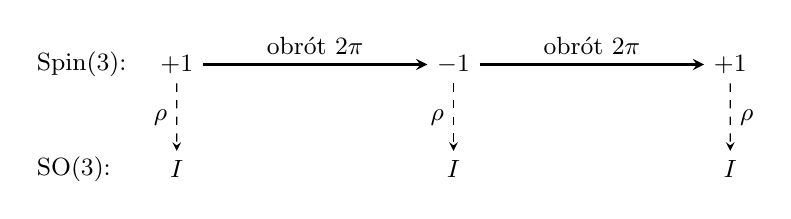
\begin{tikzpicture}[>=stealth,scale=.95,every node/.style={font=\small}]
 \node (u0) at (-3.7,1.15) {$+1$};
 \node (u1) at (0,1.15) {$-1$};
 \node (u2) at (3.7,1.15) {$+1$};
 \draw[->,thick] (u0)--node[above] {obrót $2\pi$} (u1);
 \draw[->,thick] (u1)--node[above] {obrót $2\pi$} (u2);
 \node (v0) at (-3.7,-.25) {$I$};
 \node (v1) at (0,-.25) {$I$};
 \node (v2) at (3.7,-.25) {$I$};
 \draw[->,dashed] (u0)--node[left] {$\rho$} (v0);
 \draw[->,dashed] (u1)--node[left] {$\rho$} (v1);
 \draw[->,dashed] (u2)--node[right] {$\rho$} (v2);
 \node[anchor=west] at (-5.7,1.15) {$\mathrm{Spin}(3)$:};
 \node[anchor=west] at (-5.7,-.25) {$\mathrm{SO}(3)$:};
\end{tikzpicture}

{\small\itshape Dwa pełne obroty: po $2\pi$ obrót wektorów
jest tożsamością, ale jego podniesienie do grupy Spin
ma znak minus; po $4\pi$ znak znika.}
\end{center}

Rozważmy sprzężenie z zadanym polem elektromagnetycznym.
Niech $q$ będzie ładunkiem cząstki, $\Phi$ potencjałem
skalarnym, $\mathbf A$ potencjałem wektorowym,
$\mathbf B=\nabla\times\mathbf A$ i
$\pi=-i\nabla-q\mathbf A$. Minimalne sprzężenie prowadzi
do hamiltonianu
$H=\alpha\cdot\pi+m\beta+q\Phi$.
Załóżmy najpierw, że potencjały są niezależne od czasu,
i rozważmy stan stacjonarny
$\psi(t,x)=e^{-iEt}(\varphi(x),\chi(x))^T$.
W reprezentacji~\eqref{eq:dirac-gamma-reprezentacja}
równanie $H\psi=E\psi$ jest równoważne układowi
\begin{equation}\label{eq:dirac-uklad-pauli}
 (E-q\Phi-m)\varphi=(\sigma\cdot\pi)\chi,\qquad
 (E-q\Phi+m)\chi=(\sigma\cdot\pi)\varphi.
\end{equation}
W reżimie nierelatywistycznym zakładamy
$|E-q\Phi-m|\ll m$ oraz pędy małe w porównaniu z $m$.
Drugie równanie daje wtedy w przybliżeniu
$\chi=(2m)^{-1}(\sigma\cdot\pi)\varphi$.
Nie jest to dokładna równość: zaniedbujemy poprawki
wyższego rzędu względem $1/m$.

Z relacji $\sigma_i\sigma_j=\delta_{ij}I_2+
 i\sum_k\varepsilon_{ijk}\sigma_k$ i komutatora
$[\pi_i,\pi_j]=iq\sum_k\varepsilon_{ijk}B_k$ wynika
\begin{align*}
 (\sigma\cdot\pi)^2
 &=\sum_i\pi_i^2+
  \frac{i}{2}\sum_{i,j,k}\varepsilon_{ijk}
                    \sigma_k[\pi_i,\pi_j]\\
 &=\pi^2-q\,\sigma\cdot\mathbf B.
\end{align*}
Podstawienie do pierwszej równości
\eqref{eq:dirac-uklad-pauli} daje, po odjęciu energii
spoczynkowej, równanie Pauliego w pierwszym przybliżeniu:
\begin{equation}\label{eq:dirac-pauli}
 i\partial_t\varphi
 =\left(\frac{\pi^2}{2m}+q\Phi
 -\frac{q}{2m}\,\sigma\cdot\mathbf B\right)\varphi.
\end{equation}
Tutaj $\varphi$ po prawej i lewej stronie oznacza wolno
zmieniającą się amplitudę po usunięciu fazy $e^{-imt}$.
Ostatni człon jest sprzężeniem momentu magnetycznego
ze spinem $\mathbf S=\sigma/2$. Daje czynnik $g=2$
na poziomie równania Diraca; poprawki z kwantowej teorii
pola mogą zmieniać tę wartość.

\subsection{Dokładne rozwiązanie związane: atom wodoropodobny}
\label{subsec:dirac-coulomb}

Swobodne fale płaskie nie opisują stanów związanych.
Rozważmy więc relatywistyczny elektron w statycznym,
sferycznie symetrycznym potencjale elektrostatycznym
$V(r)$, bez pola magnetycznego. Wtedy równanie
stacjonarne ma postać
\begin{equation}\label{eq:dirac-centralny}
 \left(-i\alpha\cdot\nabla+m\beta+V(r)\right)\Psi
 =E\Psi,
\end{equation}
gdzie $\alpha^j=\gamma^0\gamma^j$,
$\beta=\gamma^0$ i $r=|x|$.
Dla potencjału Coulomba $V(r)=-a/r$,
$a=Z\alpha_{\mathrm{fs}}$, przyjmujemy jądro
punktowe o ładunku $Ze$ i nieskończonej masie.
Tutaj $\alpha_{\mathrm{fs}}\approx1/137$ jest
stałą struktury subtelnej, nie macierzą Diraca.

Dla stanów o ustalonym momencie całkowitym
stosujemy dwuskładowe \emph{sferyczne spinory}
$\Omega_{\kappa\mu}$, normowane w $L^2(S^2)$, które
spełniają
$\sigma\cdot\widehat r\,\Omega_{\kappa\mu}
=-\Omega_{-\kappa,\mu}$ oraz
$(\sigma\cdot L)\Omega_{\kappa\mu}
=-(\kappa+1)\Omega_{\kappa\mu}$.
Liczba $\kappa=\pm(j+\tfrac12)$ jest niezerową
liczbą całkowitą, a $\mu=-j,\ldots,j$.
Szukamy rozwiązań postaci
\begin{equation}\label{eq:dirac-centralny-ansatz}
 \Psi(x)=\frac1r\begin{pmatrix}
 G(r)\Omega_{\kappa\mu}(\widehat r)\\
 iF(r)\Omega_{-\kappa,\mu}(\widehat r)
 \end{pmatrix}.
\end{equation}

Wykorzystując tożsamość
$\sigma\cdot(-i\nabla)
=-i(\sigma\cdot\widehat r)
  (\partial_r-r^{-1}\sigma\cdot L)$,
otrzymujemy
$\sigma\cdot(-i\nabla)
 [r^{-1}G\Omega_{\kappa\mu}]
 =ir^{-1}(G'+\kappa G/r)\Omega_{-\kappa,\mu}$.
Po podstawieniu~\eqref{eq:dirac-centralny-ansatz}
do~\eqref{eq:dirac-centralny} i porównaniu
obu dwuskładowych bloków dostajemy układ
\begin{equation}\label{eq:dirac-rownania-radialne}
 \begin{aligned}
 G'(r)+\frac\kappa rG(r)&=(m+E-V(r))F(r),\\
 F'(r)-\frac\kappa rF(r)&=(m-E+V(r))G(r).
 \end{aligned}
\end{equation}
Zamiast jednego równania Schrödingera drugiego rzędu
otrzymaliśmy układ dwóch równań pierwszego rzędu,
sprzęgających górne i dolne składowe spinora.

\begin{przyklad}[Dokładna energia i funkcja radialna stanu podstawowego]
\label{prz:dirac-coulomb-ground}
Niech $0<a<1$ i $\kappa=-1$, co odpowiada
stanowi $j=1/2$ o najmniejszym orbitalnym
momencie pędu. Połóżmy
$\gamma=\sqrt{1-a^2}$ i $\lambda=ma$.
Wtedy funkcje
\begin{equation}\label{eq:dirac-coulomb-ground}
 \begin{aligned}
 G(r)&=N\,r^{\gamma}e^{-\lambda r},\\
 F(r)&=-\frac{a}{1+\gamma}\,G(r),\\
 E&=m\gamma=m\sqrt{1-a^2}
 \end{aligned}
\end{equation}
rozwiązują układ~\eqref{eq:dirac-rownania-radialne}
dla $V(r)=-a/r$. Każdy z dwóch wyborów
$\mu=\pm1/2$ daje jeden stan o tej energii.
\end{przyklad}
\begin{proof}
Poszukajmy rozwiązania z $F=cG$ oraz
$G(r)=Nr^\gamma e^{-\lambda r}$, $\lambda>0$.
Dla $\kappa=-1$ pierwsze z równań radialnych
daje, po podzieleniu przez $G$,
$\frac{\gamma-1}{r}-\lambda
=c(m+E+a/r)$.
Drugie daje
$c\bigl(\frac{\gamma+1}{r}-\lambda\bigr)
=m-E-a/r$.
Porównując wyrazy stałe i współczynniki przy
$r^{-1}$, dostajemy cztery warunki:
\[
 \gamma-1=ac,\qquad c(\gamma+1)=-a,
 \qquad -\lambda=c(m+E),\qquad -c\lambda=m-E.
\]
Pierwsze dwa dają $\gamma^2=1-a^2$ i
$c=-a/(1+\gamma)$; dwa ostatnie prowadzą do
$c^2=(m-E)/(m+E)$, a stąd $E=m\gamma$
i $\lambda=ma$. Otrzymaliśmy więc
\eqref{eq:dirac-coulomb-ground} bez pomijania
równań wiążących obie składowe.
Ponieważ $\Omega_{\kappa\mu}$ są unormowane
na sferze, warunek $\|\Psi\|_{L^2(\mathbb R^3)}=1$
sprowadza się do
$\int_0^\infty(|G|^2+|F|^2)\,\dd r=1$.
Wystarczy więc wybrać
\[
 N=\left(\frac{(2\lambda)^{2\gamma+1}}
 {\bigl(1+a^2/(1+\gamma)^2\bigr)\,
  \Gamma(2\gamma+1)}\right)^{1/2},
\]
gdzie $\Gamma$ oznacza funkcję gamma Eulera.
Dla $0<a<1$ rozwiązanie jest całkowalne
zarówno w zerze, jak i w nieskończoności.
\end{proof}

Dla wodoru ($Z=1$) w przybliżeniu nieruchomego
jądra wzór daje
$E=m\sqrt{1-\alpha_{\mathrm{fs}}^2}
 =m-\tfrac12m\alpha_{\mathrm{fs}}^2
 +O(m\alpha_{\mathrm{fs}}^4)$.
Po odjęciu energii spoczynkowej otrzymujemy
znaną nierelatywistyczną energię wiązania
około $-13{,}6\,\mathrm{eV}$.
W pełnym rachunku dla innych liczb kwantowych
pojawiają się funkcje hipergeometryczne;
warunek ich redukcji do wielomianów daje
kolejne poziomy energetyczne. Efekty skończonej
masy i rozmiaru jądra oraz poprawki radiacyjne
wykraczają poza idealny model~\eqref{eq:dirac-centralny}.

\subsection{Koneksja spinorowa i operator Diraca na rozmaitości}
\label{subsec:dirac-koneksja}

Konstrukcja wiązki spinorowej i zasada sklejania pól
zostały opisane w~\ref{sec:pola-spinorowe-podstawy}.
Tutaj podnosimy koneksję z wiązki stycznej na
wiązkę spinorową, a następnie tworzymy operator
różniczkowy pierwszego rzędu.

Przejdźmy do geometrii riemannowskiej. Niech $(M^n,g)$
będzie zorientowaną rozmaitością ze strukturą spinową,
a $S\to M$ jej zespoloną wiązką spinorową z
Definicji~\ref{def:pole-spinorowe-globalne}.
Działanie Clifforda jest odwzorowaniem
$c:TM\to\operatorname{End}(S)$, spełniającym
$c(v)c(w)+c(w)c(v)=-2g(v,w)I$.

Koneksja Leviego--Civity na wiązce ramek ortonormalnych
jest opisana lokalnymi $\mathfrak{so}(n)$-wartościowymi
formami koneksji. Homomorfizm nakrycia
$\operatorname{Spin}(n)\to\mathrm{SO}(n)$ indukuje
\emph{izomorfizm algebr Liego} $\mathfrak{spin}(n)
\simeq\mathfrak{so}(n)$. Dzięki niemu formy koneksji
podnoszą się jednoznacznie; zgodność funkcji przejścia
zapewnia, że lokalne podniesienia sklejają się w koneksję
na wiązce głównej spinowej. Przez reprezentację spinową
otrzymujemy \emph{koneksję spinorową} $\nabla^S$.
Spełnia ona regułę Leibniza oraz
\begin{equation}\label{eq:dirac-zgodnosc}
 \nabla^S_X\bigl(c(Y)\psi\bigr)
 =c(\nabla_XY)\psi+c(Y)\nabla^S_X\psi.
\end{equation}
W lokalnej zorientowanej ramce ortonormalnej
$(e_a)_{a=1}^n$, po wyborze jej podniesienia spinowego,
możemy zapisać
\begin{equation}\label{eq:dirac-koneksja-lokalna}
 \nabla^S_{e_j}\psi
 =e_j(\psi)+\frac14\sum_{a,b=1}^n
 \omega_{jab}\,c(e_a)c(e_b)\psi,
 \qquad
 \omega_{jab}=g(\nabla_{e_j}e_a,e_b).
\end{equation}
Oznaczenie $e_j(\psi)$ dotyczy współrzędnych spinora
w wybranej lokalnej trywializacji, nie stanowi
niezależnej od ramki pochodnej spinora.
Aby zobaczyć współczynnik $1/4$, oznaczmy przez $A_j$
macierzowy człon koneksji. Ponieważ
$\omega_{jab}=-\omega_{jba}$, z relacji Clifforda
wynika
\[
 \left[\frac14\sum_{a,b}\omega_{jab}c(e_a)c(e_b),
 c(e_k)\right]=\sum_b\omega_{jkb}c(e_b).
\]
Jest to dokładnie warunek~\eqref{eq:dirac-zgodnosc}
przy zapisaniu $\nabla_{e_j}e_k=\sum_b\omega_{jkb}e_b$.
Tak otrzymuje się lokalny wzór na koneksję spinorową.
Wzór zależy od ramki, ale wyznacza globalną koneksję.

\begin{definicja}[Riemannowski operator Diraca]
\label{def:operator-diraca-riemann}
Niech $n\geq2$ i niech $(M^n,g,\mathfrak o,\mathfrak s)$
będzie riemannowską rozmaitością spinową z
Definicji~\ref{def:rozmaitosc-spinowa}. Niech $S=S(M)$
będzie jej zespoloną wiązką spinorową, a $\nabla^S$
koneksją spinorową indukowaną przez koneksję
Leviego--Civity. Operator Diraca to operator różniczkowy
pierwszego rzędu $D:\Gamma^\infty(S)\to\Gamma^\infty(S)$
zadany wzorem
\begin{equation}\label{eq:dirac-riemann}
 D\psi=\sum_{j=1}^n c(e_j)\nabla^S_{e_j}\psi,
\end{equation}
gdzie $(e_j)$ jest dowolną lokalną ramką ortonormalną.
\end{definicja}

Definicja nie zależy od ramki: jeśli $e'_j=\sum_k A_{kj}e_k$
i $A\in\mathrm{SO}(n)$, to w podwójnej sumie
pojawia się $\sum_jA_{kj}A_{\ell j}=\delta_{k\ell}$.
W odróżnieniu od równania lorentzowskiego
nie umieszczamy tutaj czynnika $i$. Dla naturalnego
hermitowskiego iloczynu na spinorach $c(e_j)^*=-c(e_j)$.
Zgodność koneksji z iloczynem hermitowskim i
z działaniem Clifforda pokazuje również formalną
samosprzężoność: dla spinorów $\psi,\phi$ o zwartym
nośniku połóżmy lokalnie
$V=\sum_j\langle\psi,c(e_j)\phi\rangle e_j$.
W ramce normalnej w rozważanym punkcie mamy
$\operatorname{div}V=
-\langle D\psi,\phi\rangle+
\langle\psi,D\phi\rangle$.
Po całkowaniu i zastosowaniu twierdzenia Stokesa
otrzymujemy
$\int_M\langle D\psi,\phi\rangle\,\dd\mu_g(x)
=\int_M\langle\psi,D\phi\rangle\,\dd\mu_g(x)$.
Na rozmaitości z brzegiem trzeba dodatkowo uwzględnić
wyraz brzegowy i warunki brzegowe.

\begin{stwierdzenie}[Eliptyczność]
\label{prop:dirac-eliptycznosc}
Niech $n\geq2$ i niech $(M^n,g,\mathfrak o,\mathfrak s)$
będzie riemannowską rozmaitością spinową. Niech
$D:\Gamma^\infty(S(M))\to\Gamma^\infty(S(M))$
będzie operatorem Diraca z
Definicji~\ref{def:operator-diraca-riemann}.
Wówczas $D$ jest operatorem eliptycznym.
\end{stwierdzenie}
\begin{proof}
Jego symbol główny w konwencji różniczkowej to
$\sigma_D(x,\xi)=c(\xi^\sharp)$.
Dzięki relacji Clifforda
$\sigma_D(x,\xi)^2=-|\xi|_g^2I$, więc dla
$\xi\ne0$ symbol jest odwracalny.
\end{proof}

\begin{przyklad}[Płaski torus i zależność od struktury spinowej]
\label{prz:dirac-torus}
Na $T^2=\mathbb R^2/(2\pi\mathbb Z)^2$ ze standardową
metryką i periodyczną strukturą spinową mamy
$S=T^2\times\mathbb C^2$ oraz
$D=i\sigma_1\partial_x+i\sigma_2\partial_y$.
Na modzie $e^{i(kx+\ell y)}u$,
$(k,\ell)\in\mathbb Z^2$, operator działa przez
macierz $-k\sigma_1-\ell\sigma_2$, o wartościach
własnych $\pm\sqrt{k^2+\ell^2}$ dla $(k,\ell)\ne(0,0)$.
Dla $(k,\ell)=(0,0)$ jądro ma wymiar $2$:
są to spinory stałe. Przy strukturze spinowej
antyperiodycznej w choć jednym kierunku odpowiedni
pęd ma postać liczby całkowitej przesuniętej o $1/2$;
mod zerowy nie istnieje, zatem $\ker D=\{0\}$.
To pokazuje, że operator Diraca pamięta nie tylko
metrykę, lecz także wybór struktury spinowej.
\end{przyklad}

\subsection{Wzór Lichnerowicza i metoda Bochnera}

Niech $\nabla^{S*}\nabla^S$ oznacza laplasjan koneksyjny,
a $\mathrm{Scal}_g$ krzywiznę skalarną w konwencji
zgodnej z Rozdziałem~\ref{ch:krzywizna}.

\begin{twierdzenie}[Wzór Schrödingera--Lichnerowicza]
\label{thm:lichnerowicz}
Niech $n\geq2$ i niech $(M^n,g,\mathfrak o,\mathfrak s)$
będzie riemannowską rozmaitością spinową. Niech
$S=S(M)$ będzie jej zespoloną wiązką spinorową,
$\nabla^S$ koneksją spinorową indukowaną przez koneksję
Leviego--Civity, $D=\sum_{j=1}^n c(e_j)\nabla^S_{e_j}$
operatorem Diraca, a $\nabla^{S*}\nabla^S$
laplasjanem koneksyjnym. Wtedy jako operatory na
$\Gamma^\infty(S)$ zachodzi
\begin{equation}\label{eq:lichnerowicz}
 D^2=\nabla^{S*}\nabla^S+\frac14\mathrm{Scal}_g\,I_S.
\end{equation}
\end{twierdzenie}
\begin{proof}
Ustalmy $p\in M$. Wybierzmy ramkę ortonormalną
normalną w $p$, czyli $\nabla_{e_i}e_j(p)=0$,
a jej wektory w $p$ dobierzmy ponadto jako wektory
własne symetrycznego tensora Ricciego.
Zgodność\,\eqref{eq:dirac-zgodnosc} daje w $p$
\begin{align*}
 D^2\psi
 &=\sum_{i,j}c(e_i)c(e_j)\nabla^S_{e_i}\nabla^S_{e_j}\psi\\
 &=-\sum_i\nabla^S_{e_i}\nabla^S_{e_i}\psi
   +\sum_{i<j}c(e_i)c(e_j)R^S(e_i,e_j)\psi.
\end{align*}
W pierwszej sumie mamy właśnie
$\nabla^{S*}\nabla^S\psi$ w punkcie $p$.
W drugiej występuje krzywizna koneksji spinorowej:
\begin{equation}\label{eq:dirac-krzywizna-spinowa}
 R^S(e_i,e_j)=\frac14\sum_{a,b}
 R_{ijab}\,c(e_a)c(e_b),\qquad
 R_{ijab}:=g(R(e_i,e_j)e_a,e_b).
\end{equation}
Otrzymujemy ją, podnosząc krzywiznę
koneksji Leviego--Civity przez izomorfizm
$\mathfrak{so}(n)\simeq\mathfrak{spin}(n)$.

Sprawdźmy teraz kontrakcję, która jest istotą wzoru.
Skróćmy $c(e_i)$ do $c_i$. Wstawienie
\eqref{eq:dirac-krzywizna-spinowa} daje
$\frac14\sum_{i<j,a,b}R_{ijab}c_ic_jc_ac_b$.
Dzielimy składniki według liczby różnych indeksów:
\begin{enumerate}
 \item Gdy wszystkie cztery indeksy są różne,
  ich współczynniki sumują się do zera dzięki
  pierwszej tożsamości Bianchiego. Dla ustalonych
  $i,j,a,b$ pojawia się kombinacja
  $R_{ijab}+R_{jaib}+R_{aijb}=0$,
  z uwzględnieniem znaków porządkowania $c$.
 \item Gdy są trzy różne indeksy, po zsumowaniu
  po indeksie powtórzonym otrzymujemy współczynniki
  proporcjonalne do pozadiagonalnych wyrazów
  $\operatorname{Ric}_{jk}$. Te są zerowe w wybranej
  ramce diagonalizującej Ricciego.
 \item Gdy zostają tylko indeksy $i,j$, mamy
  $R_{ijji}=-R_{ijij}$ oraz $c_jc_i=-c_ic_j$.
  Wówczas odpowiednia część $R^S(e_i,e_j)$ to
  $\tfrac12R_{ijij}c_ic_j$. Ponieważ $(c_ic_j)^2=-I$,
  po pomnożeniu przez $c_ic_j$ otrzymujemy
  $-\tfrac12R_{ijij}I$.
\end{enumerate}
W konwencji krzywizny z
Definicji~\ref{def:tensor-krzywizny} mamy
$\mathrm{Scal}_g=-2\sum_{i<j}R_{ijij}$.
Ostatecznie
\[
 \sum_{i<j}c_ic_jR^S(e_i,e_j)
 =-\frac12\sum_{i<j}R_{ijij}I
 =\frac14\mathrm{Scal}_g I.
\]
To daje tezę w $p$; punkt $p$ był dowolny.
\end{proof}

\begin{wniosek}[Dodatnia krzywizna skalarna wyklucza spinory harmoniczne]
\label{cor:dirac-dodatni-scalar}
Niech $n\geq2$ i niech $(M^n,g,\mathfrak o,\mathfrak s)$
będzie zwartą riemannowską rozmaitością spinową bez brzegu.
Niech $D$ będzie operatorem Diraca na $S(M)$.
Jeżeli $\mathrm{Scal}_g(x)>0$ dla każdego $x\in M$,
to $\ker D=\{0\}$.
\end{wniosek}
\begin{proof}
Dla $D\psi=0$, po scałkowaniu~\eqref{eq:lichnerowicz}
i skorzystaniu z formalnej samosprzężoności,
mamy
\[
 0=\|D\psi\|_{L^2}^2
 =\|\nabla^S\psi\|_{L^2}^2
  +\frac14\int_M\mathrm{Scal}_g|\psi|^2\,\dd\mu_g(x).
\]
Oba składniki są nieujemne, a drugi może zniknąć
tylko wtedy, gdy $\psi=0$.
\end{proof}

\subsection{Operator de Rhama i charakterystyka Eulera}

Nie należy utożsamiać operatora Diraca na spinorach
z operatorem $d+\delta$ na formach różniczkowych,
choć obie konstrukcje należą do tej samej rodziny.
Na $\Lambda^*T^*M\otimes\mathbb C$ definiujemy
działanie Clifforda
$c(v)\alpha=v^\flat\wedge\alpha-\iota_v\alpha$.
W lokalnej ramce ortonormalnej otrzymujemy
\begin{equation}\label{eq:dirac-de-rham}
 D_{\mathrm{dR}}=d+\delta
 =\sum_{j=1}^n c(e_j)\nabla_{e_j},
 \qquad D_{\mathrm{dR}}^2=\Delta_H=d\delta+\delta d.
\end{equation}
Rozkład na formy parzystego i nieparzystego stopnia
daje operator $D_{\mathrm{dR}}^+:\Omega^{\mathrm{parz}}(M)
\to\Omega^{\mathrm{nieparz}}(M)$.

\begin{stwierdzenie}[Indeks operatora de Rhama]
\label{prop:dirac-indeks-euler}
Niech $n\geq1$ i niech $(M^n,g)$ będzie zwartą,
zorientowaną rozmaitością riemannowską bez brzegu.
Niech $D_{\mathrm{dR}}^+=d+\delta$ oznacza ograniczenie
operatora $d+\delta$ z form parzystego stopnia
na formy nieparzystego stopnia. Wówczas
\begin{equation}\label{eq:dirac-indeks-euler}
 \operatorname{ind}D_{\mathrm{dR}}^+
 =\sum_{k=0}^n(-1)^k\dim H^k_{\mathrm{dR}}(M)
 =\chi(M).
\end{equation}
\end{stwierdzenie}
\begin{proof}
Operator $D_{\mathrm{dR}}=d+\delta$ jest formalnie
samosprzężony i zamienia parzystość stopnia.
Jądra $D_{\mathrm{dR}}^+$ oraz jego operatora
sprzężonego składają się odpowiednio z harmonicznych
form parzystych i nieparzystych. Dokładniej,
z $d^2=\delta^2=0$ i wzajemnej sprzężoności
$d,\delta$ wynika po całkowaniu
$\|D_{\mathrm{dR}}\alpha\|^2
=\|d\alpha\|^2+\|\delta\alpha\|^2$
(także dla form niejednorodnych). Ponadto
$\langle\Delta_H\alpha,\alpha\rangle
=\|d\alpha\|^2+\|\delta\alpha\|^2$.
Otrzymujemy więc równoważność
$D_{\mathrm{dR}}\alpha=0$
i $\Delta_H\alpha=0$.
Twierdzenie Hodge'a utożsamia przestrzeń harmonicznych
$k$-form z $H^k_{\mathrm{dR}}(M)$; różnica wymiarów
jądra i kokernela daje prawą stronę~\eqref{eq:dirac-indeks-euler}.
\end{proof}

Twierdzenie Cherna--Gaussa--Bonneta z części o
klasach charakterystycznych stwierdza
\begin{equation}\label{eq:dirac-chern-gauss-bonnet}
 \chi(M)=\langle e(TM),[M]\rangle
 =\int_M\operatorname{Pf}\!\left(\frac{\Omega}{2\pi}\right)
\end{equation}
dla zwartej zorientowanej rozmaitości parzystego
wymiaru, przy odpowiednio znormalizowanej macierzy
form krzywizny $\Omega$ w ramce ortonormalnej.
Prawa strona jest geometrycznym całkowym wyrażeniem
charakterystyki Eulera. Połączenie jej z
\eqref{eq:dirac-indeks-euler} daje równość
\[
 \operatorname{ind}D_{\mathrm{dR}}^+
 =\langle e(TM),[M]\rangle.
\]
W wymiarze nieparzystym charakterystyka Eulera
zamkniętej zorientowanej rozmaitości jest zerowa,
co wynika też z dualności Poincarégo.

Jest to szczególny przypadek formuły indeksowej
Atiyaha--Singera. Sama tożsamość Hodge'a i twierdzenie
Cherna--Gaussa--Bonneta nie stanowią dowodu ogólnego
twierdzenia indeksowego dla wszystkich operatorów
eliptycznych; pokazują natomiast jego treść w tej
konkretnej sytuacji. W przypadku powierzchni
$\int_M e(TM)=(2\pi)^{-1}\int_M K\,\dd\mu_g(x)$, co sprowadza
powyższą równość do klasycznej formuły Gaussa--Bonneta.

\subsection{Chiralny operator Diraca i rodzaj \texorpdfstring{$\widehat A$}{A-hat}}

Niech $M^{2m}$ będzie zwartą, zorientowaną
rozmaitością spinową bez brzegu.
W Rozdziale~\ref{ch:grass-spin} zdefiniowaliśmy
rozkład na półspinory $S=S^+\oplus S^-$.
Wolumenowy operator chiralności $\Gamma$ jest
równoległy ($\nabla^S\Gamma=0$), gdyż koneksja
Leviego--Civity zachowuje metrykę i orientację.
Antykomutuje z $c(v)$ dla każdego wektora $v$.
Stąd $D\Gamma=-\Gamma D$, a więc mnożenie Clifforda
przez wektor i sam operator $D$ zamieniają
obie części. Operator $D$ ma postać
\[
 D=\begin{pmatrix}0&D^-\\D^+&0\end{pmatrix},
 \qquad D^+:\Gamma(S^+)\longrightarrow\Gamma(S^-).
\]
Na zwartej rozmaitości eliptyczność i twierdzenia
o regularności eliptycznej zapewniają skończoną
wymiarowość jąder (i własność Fredholma).
Formalna samosprzężoność $D$ daje $(D^+)^*=D^-$. Indeks analityczny jest liczbą całkowitą
$\operatorname{ind}D^+=\dim\ker D^+-\dim\ker D^-$.
Twierdzenie indeksowe Atiyaha--Singera, zastosowane
do operatora spinowego, daje
\begin{equation}\label{eq:dirac-ahat}
 \operatorname{ind}D^+=\langle\widehat A(TM),[M]\rangle.
\end{equation}
Tutaj $\widehat A(TM)$ jest klasą charakterystyczną
wyrażalną przez klasy Pontriagina; jej początkowe
składniki to
$\widehat A=1-\tfrac1{24}p_1
+\tfrac1{5760}(7p_1^2-4p_2)+\cdots$.
Wymiar $4$ daje w szczególności
$\operatorname{ind}D^+=-\langle p_1(TM),[M]\rangle/24$.

\begin{wniosek}[Topologiczna przeszkoda do dodatniej krzywizny skalarnej]
\label{cor:dirac-ahat-dodatni-scalar}
Niech $k\geq1$ będzie liczbą całkowitą i niech
$(M^{4k},g,\mathfrak o,\mathfrak s)$ będzie zwartą,
zorientowaną riemannowską rozmaitością spinową bez brzegu.
Jeżeli $\mathrm{Scal}_g(x)>0$ dla każdego $x\in M$,
to $\langle\widehat A(TM),[M]\rangle=0$,
gdzie $\widehat A(TM)$ jest rodzajem $\widehat A$
wiązki stycznej, a $[M]\in H_{4k}(M;\mathbb Z)$
klasą fundamentalną wyznaczoną przez $\mathfrak o$.
\end{wniosek}
\begin{proof}
Wniosek~\ref{cor:dirac-dodatni-scalar} daje
$\ker D^+=\ker D^-=\{0\}$, zatem indeks jest
zerowy. Teraz stosujemy~\eqref{eq:dirac-ahat}.
\end{proof}

Warto podkreślić różnicę: operator $D_{\mathrm{dR}}$
istnieje na każdej rozmaitości riemannowskiej
i koduje kohomologię de Rhama oraz charakterystykę
Eulera; operator $D$ na \emph{spinorach} wymaga
struktury spinowej, a jego indeks wyraża rodzaj
$\widehat A$. Ta wspólna perspektywa indeksowa
nie oznacza utożsamienia obu operatorów.

\begin{center}
\begin{tikzpicture}[>=stealth,every node/.style={font=\small,align=center}]
 \node[draw,rounded corners,inner sep=7pt] (top) at (0,2)
   {operator pierwszego rzędu typu $c\circ\nabla$};
 \node[draw,rounded corners,inner sep=6pt] (left) at (-3.1,.75)
   {$D_{\mathrm{dR}}=d+\delta$\\na formach};
 \node[draw,rounded corners,inner sep=6pt] (right) at (3.1,.75)
   {$D$\\na spinorach};
 \node[draw,rounded corners,inner sep=6pt] (ll) at (-3.1,-.75)
   {$\operatorname{ind}D^+_{\mathrm{dR}}=\chi(M)$\\Chern--Gauss--Bonnet};
 \node[draw,rounded corners,inner sep=6pt] (rr) at (3.1,-.75)
   {$\operatorname{ind}D^+=\widehat A(M)$\\Atiyah--Singer};
 \draw[->] (top)--(left);
 \draw[->] (top)--(right);
 \draw[->] (left)--(ll);
 \draw[->] (right)--(rr);
\end{tikzpicture}

{\small\itshape Dwa operatory typu Diraca i dwa różne
niezmienniki topologiczne; $\widehat A(M)$ oznacza
liczbę $\langle\widehat A(TM),[M]\rangle$.}
\end{center}

\subsection{Równanie Diraca w metryce FLRW}

Rozważmy teraz zorientowaną i czasowo zorientowaną
czterowymiarową czasoprzestrzeń lorentzowską
$(\mathcal M,g)$ ze strukturą spinową. W lokalnej ramce ortonormalnej $e_a$ o sygnaturze
$(-,+,+,+)$, z dualną koramką $\theta^a$, piszemy
$\gamma^a=c(\theta^a)$; działanie na koramce spełnia
$\gamma^a\gamma^b+\gamma^b\gamma^a=-2\eta^{ab}I$.
To ważne rozróżnienie: dla wektora czasowego
$e_0$ mamy $e_0^\flat=-\theta^0$, a więc
$c(e_0)=-\gamma^0$, nie $+\gamma^0$.
Koneksja spinorowa jest podniesieniem koneksji
Leviego--Civity. Lorentzowskie równanie Diraca ma postać
\begin{equation}\label{eq:dirac-zakrzywiony}
 \left(i\sum_{a=0}^3\gamma^a\nabla^S_{e_a}-m\right)\psi=0.
\end{equation}
W przeciwieństwie do operatora riemannowskiego
jego część różniczkowa nie jest eliptyczna:
symbol główny staje się osobliwy na niezerowych
kowektorach zerowych (świetlnych). Równanie to
jest równaniem ewolucji typu hiperbolicznego;
nie stosujemy do niego bezpośrednio twierdzenia
Atiyaha--Singera przeznaczonego dla operatorów
eliptycznych na zwartych rozmaitościach.

\begin{przyklad}[Dirac w przestrzennie płaskim modelu FLRW]
\label{prz:dirac-flrw}
Niech $\mathcal M=I\times\mathbb R^3$,
$g=-dt^2+a(t)^2(dx^2+dy^2+dz^2)$, gdzie
$a(t)>0$, i oznaczmy $H(t)=\dot a(t)/a(t)$.
Wybierzmy ortonormalną ramkę
$e_0=\partial_t$, $e_j=a^{-1}\partial_j$.
W koramce dualnej mamy
$\theta^0=dt$, $\theta^j=a(t)dx^j$.
Z metryki wynika
$[e_0,e_j]=-He_j$ oraz $[e_i,e_j]=0$.
Wstawienie tych relacji do wzoru Koszula daje
$\nabla_{e_0}e_a=0$,
$\nabla_{e_j}e_0=He_j$
oraz $\nabla_{e_j}e_k=H\delta_{jk}e_0$.
W konsekwencji na koramce
$\nabla_{e_j}\theta^0=-H\theta^j$ i
$\nabla_{e_j}\theta^k=-H\delta_{jk}\theta^0$.

Niech $A_j$ oznacza macierzowy składnik koneksji
spinorowej w kierunku $e_j$. Zgodność
$\nabla^S(c(\theta)\psi)
=c(\nabla\theta)\psi+c(\theta)\nabla^S\psi$
wymaga
$[A_j,\gamma^0]=-H\gamma^j$ i
$[A_j,\gamma^k]=-H\delta_{jk}\gamma^0$.
Relacje Clifforda pokazują, że spełnia je
$A_j=\tfrac H2\gamma^0\gamma^j$.
Tak więc w wybranej lokalnej trywializacji
\[
 \nabla^S_{e_0}=\partial_t,
 \qquad
 \nabla^S_{e_j}=a^{-1}\partial_j
   +\frac H2\gamma^0\gamma^j.
\]
Ponieważ $\gamma^j\gamma^0\gamma^j=\gamma^0$,
każdy kierunek przestrzenny wnosi do operatora
$\gamma^j\nabla^S_{e_j}$ dokładnie
$\tfrac H2\gamma^0$. Suma trzech takich składników
prowadzi do członu $\tfrac32H\gamma^0$.
Zsumowanie wszystkich kierunków w
\eqref{eq:dirac-zakrzywiony} daje
\begin{equation}\label{eq:dirac-flrw}
 \left[i\gamma^0\left(\partial_t+\frac32H\right)
 +\frac{i}{a(t)}\sum_{j=1}^3\gamma^j\partial_j-m\right]\psi=0.
\end{equation}
Wprowadzenie $\chi(t,x)=a(t)^{3/2}\psi(t,x)$
usuwa człon $3H/2$:
\begin{equation}\label{eq:dirac-flrw-reskalowanie}
 \left(i\gamma^0\partial_t
 +\frac{i}{a(t)}\sum_{j=1}^3\gamma^j\partial_j-m\right)\chi=0.
\end{equation}
W czasie konforemnym $\dd\tau=\dd t/a(t)$
równanie przyjmuje postać
\[
 \left(i\gamma^0\partial_\tau
 +i\sum_{j=1}^3\gamma^j\partial_j-ma(\tau)\right)\chi=0.
\]
Dla $m=0$ jest to zwykłe płaskie równanie
Diraca. Wynik odzwierciedla konforemną
niezmienniczość bezmasowego równania Diraca
w wymiarze $4$. Jeśli $a(t)\to0$ na brzegu $I$,
przekształcenie nie dowodzi jednak przedłużalności
metryki ani fizycznego rozwiązania przez taki brzeg:
może tam występować rzeczywista osobliwość
czasoprzestrzeni.
\end{przyklad}

\begin{uwaga}[Dwie geometrie i dwa typy problemów]
W fizyce relatywistycznej pytamy o propagację
fermionów, prąd zachowany i oddziaływanie z polem
oraz krzywizną czasoprzestrzeni. W geometrii
riemannowskiej pytamy o jądro i widmo operatora
eliptycznego, formułę Lichnerowicza oraz indeks.
Obie sytuacje mają wspólną algebrę Clifforda i
reprezentację spinową, lecz różnią się sygnaturą
metryki i typem analitycznym operatora.
\end{uwaga}

% <<<<<<<<<<<<< CODEX: KONIEC ROZDZIAŁU 28
